% Generated by scripts/build_venue_latex.py from Precis_paper_clean_plane_revised_v10.docx -- do not edit by hand.
\documentclass[journal]{IAENGtran}
\usepackage[T1]{fontenc}
\usepackage[utf8]{inputenc}
\usepackage{mathptmx}
\usepackage{textcomp}
\usepackage{amsmath,amssymb}
\usepackage{graphicx}
\usepackage{array}
\usepackage{adjustbox}
\usepackage{listings}
\usepackage{seqsplit}
\usepackage{tikz}
\usetikzlibrary{positioning,arrows.meta,shapes.geometric,fit,calc}
\usepackage{url}
\lstset{literate={←}{{$\leftarrow$}}1 {é}{{\'e}}1}
\usepackage{newunicodechar}
\newunicodechar{−}{\textminus}
\newunicodechar{×}{\texttimes}
\newunicodechar{≈}{\ensuremath{\approx}}
\newunicodechar{‑}{-}
\setlength{\emergencystretch}{1.5em}
\usepackage{cite}
\newcommand{\leadin}[1]{\textit{#1}}
\hyphenation{Pré-cis}
\begin{document}
\title{Keeping Tables Intact Under a Token Budget: Structure, Simple Baselines and Answer Format in Local Retrieval-Augmented Question Answering}
\author{Chandan D, M P Jeevan Gowda, Bhimsen and Chandu S%
\thanks{Manuscript received October 22, 2026. This work received no specific funding; the authors declare no competing interests.}%
\thanks{Chandan D is a final-year undergraduate student in the Department of Artificial Intelligence and Machine Learning, Impact College of Engineering and Applied Sciences, Bengaluru, India (corresponding author; e-mail: chandanxdev@gmail.com). M P Jeevan Gowda is a final-year undergraduate student in the Department of Artificial Intelligence and Machine Learning, Impact College of Engineering and Applied Sciences, Bengaluru, India (e-mail: mpjeevangowda@gmail.com). Bhimsen is a final-year undergraduate student in the Department of Artificial Intelligence and Machine Learning, Impact College of Engineering and Applied Sciences, Bengaluru, India (e-mail: harishbhimsen12396@gmail.com). Chandu S is a final-year undergraduate student in the Department of Artificial Intelligence and Machine Learning, Impact College of Engineering and Applied Sciences, Bengaluru, India (e-mail: kingskingchandu143@gmail.com).}}
\maketitle
\pagestyle{empty}
\thispagestyle{empty}
\begin{abstract}
Retrieval-augmented generation on local hardware must fit evidence into a small context, and pages whose answers sit in tables raise the question of how much of their structure to keep. We study it with Précis, an offline pipeline that keeps HTML tables and lists in native form and packs them first under an estimated-token ceiling with a guarded structural-priority rule (G), against cheap baselines on table-bearing Natural Questions pages. On short pages, the system's own rewrite of tables as extracted sentences cut exact match (EM) to 14.0\%, against 49.5\% for native tables (in-sample); against tag-stripped chunks, the cheap structure-keeping baselines were never significantly ahead (−2.5 to +6.0 points at the 2,048 ceiling on the protocol-first cohorts). On a fresh cohort G (48.0\% EM) was level with raw-markup, table-aware and hybrid chunks and whole-document Markdown (47.0 to 49.0\%), with three generators from two model families. On 200 full Wikipedia pages, where the 2,048-token ceiling binds, G was the worst arm (22.0\% EM against 33.0 to 41.5\%): same-document fact suppression removed every prose fact, leaving lists and reference text in half-filled contexts; a repaired rule (G2) raised EM on a fresh draw from 17.5\% to 33.5\%, non-inferior to table-aware chunking. A short-answer prompt format raised EM by 25.0 to 36.5 points, but a language-model judge, checked against two blind author labellers (92\% and 97\% agreement), saw gains of 1.5 to 12.0 points. Native structure should be kept but not at the expense of prose, and strict-match comparisons conflate answer format with accuracy.
\end{abstract}
\begin{IAENGkeywords}
Answer-Format Sensitivity, Context Budget, Evaluation Methodology, Non-inferiority, Retrieval-Augmented Generation, Table Question Answering.
\end{IAENGkeywords}
\IAENGpeerreviewmaketitle

\section{Introduction}\label{sec:intro}

Retrieval-augmented generation (RAG) systems retrieve text passages and place them in a language-model prompt \cite{r1,r2}. On local hardware, small generators and limited memory favour short prompts, and long contexts are used unevenly \cite{r3}, so evidence has to be selected under a budget; this paper treats that budget as a design parameter (2,048 estimated tokens in most experiments), not as a measured hardware limit. Documents whose answers live in tables and lists make the selection harder: a table cell has meaning only through its row and column headers, and chunking, stripping markup or rewriting a table as sentences can sever those links.

This paper asks how much a structure-aware packing rule adds over simple baselines that also keep structure, and how much of a measured difference between such systems is an artefact of answer format. The testbed is Précis, an offline pipeline that keeps HTML tables and lists in native form, packs them first under an estimated-token ceiling with a guarded structural-priority rule (Candidate G), and fills any remaining budget with subject–verb–object–adjunct (SVOA) facts extracted from prose. No experiment isolates the fact layer's contribution inside G, to which it added only 111 facts over 200 contexts; where the fact-only configuration (Précis v3) was compared with plain chunks (Sections~\ref{sec:6.6} and \ref{sec:6.7}) it was behind, and an audit (Section~\ref{sec:6.8}) found its negation flag unreliable. Its specification is in Appendix B.

Three research questions guide the evaluation. RQ1 (structure and baselines): for table- and list-bearing pages, how does native-structure packing compare with structure-destroying conversion and with cheap structure-keeping baselines, and what happens when the ceiling binds? RQ2 (answer format): how much of a strict-match difference between prompts comes from answer format and how much from the abstention instruction, and does an answer-equivalence measure change the conclusion? RQ3 (information loss): at which stage is answer-bearing evidence lost?

The contributions are evaluative: (i) an ablation showing that the system's own rewrite of tables as extracted sentences is the main source of loss on a table-bearing cohort (in-sample for G), and no significant advantage of the cheap structure-keeping baselines over tag-stripped chunks on the protocol-first cohorts; (ii) a protocol-first comparison on a fresh cohort against five simple baselines, with non-inferiority verdicts over margins of 3 to 7 points, table and list strata, exploratory ceiling sweeps over single documents and five-document corpora, and a protocol-first cohort of full Wikipedia pages on which the ceiling binds; (iii) a 2×2 decomposition of a concise-answer prompt into answer format and abstention wording, scored by exact match and by an answer-equivalence judge checked against human labels; (iv) a stage-loss trace on two cohorts; and (v) negative results on the fact layer: its fact-only contexts are behind plain chunks and its negation labels are unreliable. Extending \cite{r24} and HtmlRAG \cite{r25}, the study sets a structure-first rule against table-aware, hybrid and whole-document baselines on the same table-bearing questions under one budget, including full pages, and separates answer format from abstention wording. The pipeline, protocols, per-case records and scripts are released (Data and Code Availability).

Section~\ref{sec:related} reviews related work, Section~\ref{sec:problem} formulates the packing problem, Sections~\ref{sec:system} and \ref{sec:framework} describe the system, Section~\ref{sec:results} reports results, discussion and limitations, and Section~\ref{sec:conclusions} concludes. Appendix A gives the prompt templates and Appendix B the fact-layer specification and implementation notes.

\section{Related Work}\label{sec:related}

Related work is grouped into seven themes: retrieval-augmented generation and its context limits, context compression, retrieval granularity, tables and HTML as evidence, epistemic status in text, hierarchical and hybrid retrieval, and answer evaluation and prompt sensitivity. Table~\ref{tab:1} summarises the studies reviewed.

The original RAG formulation couples a parametric sequence-to-sequence model with a retrieved non-parametric memory \cite{r1}, and dense dual-encoder retrieval became its standard front end \cite{r4}. A survey catalogues the retrieval, augmentation and generation variants \cite{r2}. Liu et al. show that accuracy degrades when relevant evidence sits in the middle of a long input \cite{r3}, and Barnett et al. catalogue failure points of engineered RAG systems, among them chunking and retrieval choices \cite{r5}. Self-RAG trains a model to decide when to retrieve and to critique its output \cite{r6}; such systems assume a model that can be fine-tuned or a window that is generous. Long-context models outperform RAG on average when well resourced, at a much higher cost \cite{r7}, retrieval helps even models with extended windows \cite{r8}, and adding retrieved passages to a long-context model can lower its accuracy \cite{r36}; whole-document input is therefore one of the baselines here.

Context compression reduces the prompt directly. LLMLingua prunes tokens using a small language model and a budget controller \cite{r9}; Selective Context removes lexical units with low self-information \cite{r10}; and RECOMP compresses retrieved documents into short summaries \cite{r11}. All three need an additional neural model at inference time, and none treats a table as a unit to be kept or dropped whole.

A second family changes the unit of retrieval. Dense X Retrieval shows that indexing propositions rather than passages can improve retrieval and downstream question answering \cite{r12}, and FActScore uses atomic facts to evaluate generated text \cite{r13}. GraphRAG builds an entity graph and community summaries for corpus-level questions \cite{r14}, at the cost of many LLM calls during indexing. Element-based chunking, which splits a document at its titles, tables and list items, improved RAG on financial reports \cite{r37}; the table-aware baseline TC of Section~\ref{sec:6.3} follows that idea. Open information extraction supplies classical machinery for tuples \cite{r15,r16,r17,r18}.

Tables are a third kind of evidence. Table question answering is usually studied with semantic parsers or table-pretrained encoders \cite{r19,r20}, which presuppose a clean table; open-domain question answering over tables, and over tables and text, adds table retrieval \cite{r21,r22}, and TableRAG retrieves schema and cell information so that a model can reason over very large tables \cite{r23}. Sui et al. benchmark how the serialisation of a table in the prompt, including markup-based formats, changes what language models can answer \cite{r24}, and HtmlRAG keeps cleaned and pruned HTML for retrieved web pages and, under a fixed context window, finds it better than plain-text and Markdown conversions and than chunk-based refiners on several question-answering sets, Natural Questions among them \cite{r25}. A general RAG pipeline receives HTML in which tables and prose are mixed, and what it does with a table before prompting decides what the generator can use. None of them compares a structure-first packing rule with table-aware and hybrid chunking and whole-document Markdown on the same table-bearing questions under one token budget, or examines such a rule on long pages where that budget binds. Précis addresses that preprocessing and packing step rather than the table-reading model.

Finally, the epistemic status of a claim has a long history. FactBank annotates event factuality along source, polarity and certainty \cite{r26}, NegEx popularised rule-based negation detection with trigger terms and scope windows \cite{r27}, and the $\ast$SEM 2012 shared task addressed negation scope and focus \cite{r28}. Précis keeps a small, closed set of modalities and rule-based negation because both are cheap, inspectable and runnable on a CPU.

Retrieval can also be hierarchical or hybrid. RAPTOR builds a tree of recursive summaries and retrieves across its levels \cite{r29}; Précis instead uses the document's own markup and no learned summaries. Combining lexical and dense rankings is a standard, strong and cheap baseline: BM25 \cite{r30} fused with a dense ranking by reciprocal rank fusion \cite{r31}; a cross-encoder reranker \cite{r32} is a stronger and costlier second stage that is not evaluated here. Section~\ref{sec:6.3} therefore compares G with table-aware chunking and a hybrid retriever, not only with plain chunking.

Evaluation choices matter as much as retrieval choices. Token-level metrics such as exact match undercount correct answers \cite{r33}, model-judged answer equivalence tracks human judgement more closely \cite{r34}, although language-model judges have known position and verbosity biases \cite{r38}, and language-model accuracy can move by tens of points with small changes of prompt format \cite{r35}. RQ2 is positioned against this work.

\begin{table*}[!t]
\centering\renewcommand{\arraystretch}{1.15}\footnotesize
\caption{Summary of related studies and the position of this work.}\label{tab:1}
\begin{adjustbox}{max width=\textwidth}
\begin{tabular}{>{\raggedright\arraybackslash}p{0.22\textwidth}>{\raggedright\arraybackslash}p{0.32\textwidth}>{\raggedright\arraybackslash}p{0.38\textwidth}}
\hline
\textbf{Study} & \textbf{Focus} & \textbf{Technique} \\
\hline
Lewis et al. \cite{r1} & Retrieval-augmented generation & Dense retrieval + seq2seq generator \\
Liu et al. \cite{r3} & Use of long contexts & Position-sensitivity analysis \\
Barnett et al. \cite{r5} & Failure points in RAG engineering & Case-study analysis \\
Jiang et al. \cite{r9} & Prompt compression & Small-LM token pruning with budget controller \\
Li et al. \cite{r10} & Context compression & Self-information filtering of lexical units \\
Xu et al. \cite{r11} & Compressing retrieved documents & Extractive and abstractive compressors \\
Chen et al. \cite{r12} & Retrieval granularity & Propositions as retrieval units \\
Tan et al. \cite{r25} & HTML as retrieved knowledge & HTML cleaning and block-tree pruning \\
Pasupat \& Liang \cite{r19}; Herzig et al. \cite{r20} & Table question answering & Semantic parsing; table-pretrained encoder \\
Chen et al. \cite{r23} & Very large tables & Schema and cell retrieval \\
Saurí \& Pustejovsky \cite{r26} & Event factuality & Annotated corpus (source, polarity, certainty) \\
Sui et al. \cite{r24} & Table serialisation for LLMs & Benchmark of input formats \\
Herzig et al. \cite{r21} & Open-domain QA over tables & Dense table retrieval \\
Sarthi et al. \cite{r29} & Hierarchical retrieval & Recursive summary tree \\
Bulian et al. \cite{r33}; Kamalloo et al. \cite{r34} & Answer-equivalence evaluation & Learned and LLM-based matching \\
Sclar et al. \cite{r35} & Prompt-format sensitivity & Format-spread analysis \\
Jin et al. \cite{r36} & Long-context models in RAG & Effect of more retrieved passages \\
Jimeno Yepes et al. \cite{r37} & Chunking for RAG & Element-type chunking \\
Zheng et al. \cite{r38} & LLM-as-a-judge & Agreement and bias analysis of LLM judges \\
This work & Structure-preserving local RAG under a budget & Native tables and lists, guarded packing; format–abstention decomposition \\
\hline
\end{tabular}
\end{adjustbox}
\end{table*}

\section{Problem Formulation}\label{sec:problem}

A document is split into prose and structural elements. A structural element e is a table or list rendered in native form, with its own embedding and source document d(e). Each prose sentence yields zero or more facts t = (s, v, o, X, n, $\mu$, a): subject, verb phrase, object, a set of typed adjuncts, a negation flag n, an epistemic modality $\mu$ $\in$ \{asserted, attributed, conditional, hypothetical\} and, for attributed facts, the source a. Facts and elements are embedded into 384-dimensional unit vectors, and facts are stored in a set G. Table~\ref{tab:2} lists the notation.

\begin{table}[!t]
\centering\renewcommand{\arraystretch}{1.15}\footnotesize
\caption{Notation used in the problem formulation.}\label{tab:2}
\begin{adjustbox}{max width=\columnwidth}
\begin{tabular}{>{\raggedright\arraybackslash}p{0.36\columnwidth}>{\raggedright\arraybackslash}p{0.58\columnwidth}}
\hline
\textbf{Symbol} & \textbf{Meaning} \\
\hline
\textit{t} = (\textit{s}, \textit{v}, \textit{o}, \textit{X}, \textit{n}, \textit{$\mu$}, \textit{a}) & SVOA fact: subject, verb, object, adjuncts, negation flag, modality, attribution \\
\textit{G}, \textit{e}\textit{\textsubscript{t}} & Fact store and the 384-d embedding of fact \textit{t} \\
\textit{SDH(t)} & Semantic Density Heuristic score of fact t (Appendix B) \\
\textit{q}, sim(\textit{t},\textit{q}) & Question and cosine similarity between a fact (or element) and the question \\
\textit{$\pi$}(\textit{t},\textit{q}), \textit{$\omega$}(\textit{t}), \textit{$\tau$}(\textit{t}) & Pack score; word count of the rendered fact; its estimated token cost \\
\textit{B} & Token ceiling (2,048 in the controlled experiments) \\
\textit{C}, $\mathcal{P}$ & Candidate facts after retrieval and filtering; packed subset \\
\textit{e}, \textit{d}(\textit{e}), \textit{$\sigma$}(\textit{e},\textit{q}) & Structural element, its source document, and its structural rank score \\
\textit{T}\textit{\textsubscript{F}}, \textit{T}\textit{\textsubscript{G}}, $\Delta$ & Mean estimated context tokens of variants F and G; relative reduction \\
\hline
\end{tabular}
\end{adjustbox}
\end{table}

Each fact carries an intrinsic score SDH(t) $\in$ [0, 1], an equally weighted sum of entity relatedness, verb informativeness, uniqueness and adjunct density (Appendix B, see~(\ref{eq:B1})); its constants were set by hand and were neither tuned nor ablated. At query time a fact is ranked by the product of this score and its relevance to the question:

\begin{equation}\label{eq:1}
\pi(t,q)=\mathrm{SDH}(t)\cdot \mathrm{sim}(t,q),\qquad \mathrm{sim}(t,q)=1-d_{\cos}(e_t,e_q)
\end{equation}

The token cost of a fact is estimated from its rendered word count \textit{$\omega$}(\textit{t}), including the negation marker, adjuncts, modality tags and the “Fact \textit{N}:” label. The 1.3 factor is a word-count proxy and was not calibrated against the generator’s own tokenizer:

\begin{equation}\label{eq:2}
\tau(t)=\max\bigl(3,\ \lfloor 1.3\,\omega(t)\rfloor+2\bigr)
\end{equation}

Selecting the fact context is a 0/1 knapsack problem over the candidates C, which the system solves greedily in descending order of $\pi$ (not of the value density $\pi$/$\tau$, which was not evaluated):

\begin{equation}\label{eq:3}
\max_{\mathcal{P}\subseteq C}\ \sum_{t\in\mathcal{P}}\pi(t,q)\quad\text{subject to}\quad \sum_{t\in\mathcal{P}}\tau(t)\le B
\end{equation}

\leadin{Structural priority (Candidate G).}  Let \textit{D}\textsubscript{$\mathcal{P}$} be the source documents of the facts packed by (\ref{eq:3}) and \textit{d}$'$ the source document of the top-ranked packed fact. A structural element \textit{e} is relevant if sim(\textit{e},\textit{q}) $\geq$ 0.25, or if it shares a keyword with the question and sim(\textit{e},\textit{q}) $\geq$ 0.15. It is eligible if \textit{d}(\textit{e}) $\in$ \textit{D}\textsubscript{$\mathcal{P}$}, if no fact was packed, or if sim(\textit{e},\textit{q}) $\geq$ 0.40. Eligible elements are ranked by similarity with a document-affinity bonus, and at most three are selected:

\begin{equation}\label{eq:4}
\begin{split}\sigma(e,q)=\mathrm{sim}(e,q)\,\bigl(1&+0.15\cdot\mathbf{1}[d(e)\in D_{\mathcal{P}}]\\&+0.10\cdot\mathbf{1}[d(e)=d']\bigr)\end{split}
\end{equation}

Selected elements are packed first, within \textit{B}. If at least one is packed, every fact whose source document contributed a packed element is suppressed, as is every fact whose subject and object both occur in the packed structural text, and the remaining budget is filled with the other facts. If nothing structural fits, the context falls back to the fact-only packing of (\ref{eq:3}). The relative context reduction of G with respect to the persistent baseline F is the descriptive quantity

\begin{equation}\label{eq:5}
\Delta=1-\frac{T_G}{T_F},\qquad T_V=\frac{1}{N}\sum_{i=1}^{N}\tau_V(i)
\end{equation}

\noindent where $\tau$\textit{\textsubscript{V}}(\textit{i}) is the estimated context tokens of variant \textit{V} on case \textit{i}. Problem statement. Given a document collection, a question \textit{q} and a hardware profile that fixes \textit{B}, construct the fact store \textit{G} and the structural store offline, then return a context of at most \textit{B} estimated tokens, built from packed structural elements and a packed subset of facts chosen greedily for a high $\Sigma$ $\pi$(t,q) while excluding hypothetical facts, and render it as a grounded prompt for a local language model. The ceiling B is enforced on estimated tokens (see~(\ref{eq:2})); the generator's own count runs about 1.24 times higher (Section~\ref{sec:6.2}), so B bounds the estimate and not the native prompt length.

\section{System Model}\label{sec:system}

\begin{figure}[!t]
\centering
% Figure 1: system architecture (Sections IV and V; stage numbers as in Section V). Drawn at print size: labels are
% 8 pt on 9.5 pt, set explicitly (jucs2e makes \footnotesize 9 pt); about 170 pt wide, so it fits one EL
% column and one half of the J.UCS figure pair at 100%.
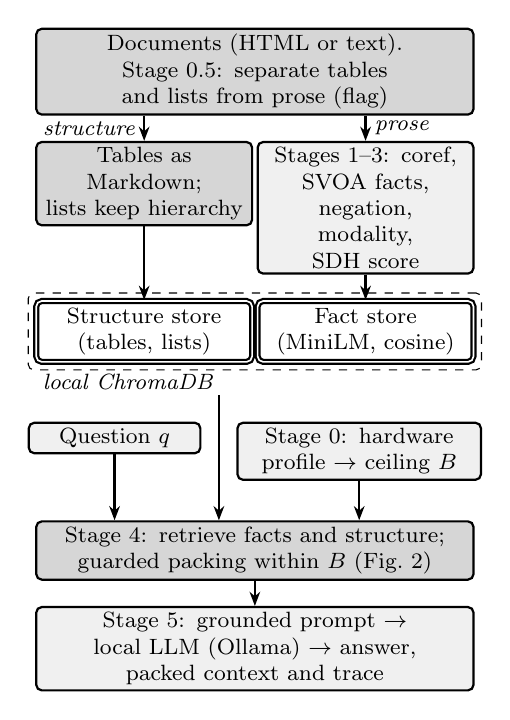
\begin{tikzpicture}[
  font=\fontsize{8}{9.5}\selectfont, >={Stealth[length=1.8mm]}, node distance=3.2mm and 3mm,
  box/.style={draw, thick, rounded corners=2pt, align=center, inner sep=2pt, fill=black!6, text width=#1,
    execute at begin node={\hyphenpenalty=10000\exhyphenpenalty=10000}},
  box/.default=74pt,
  sbox/.style={box=#1, fill=black!16}, sbox/.default=74pt,
  store/.style={box=#1, fill=white, double, double distance=0.6pt}, store/.default=74pt,
  ar/.style={->, thick},
  lab/.style={font=\fontsize{8}{9.5}\selectfont\itshape, inner sep=1pt}]
% ---------------- ingestion, once per document
\node[sbox=154pt] (split) {Documents (HTML or text). Stage 0.5: separate tables and lists from prose (flag)};
\node[sbox, below=of split.south west, anchor=north west] (md) {Tables as Markdown;\\ lists keep hierarchy};
\node[box, below=of split.south east, anchor=north east] (fact) {Stages 1--3: coref,\\ SVOA facts, negation,\\ modality, SDH score};
\node[store, below=of fact, minimum height=22pt] (fs) {Fact store\\ (MiniLM, cosine)};
\node[store, minimum height=22pt] (ss) at (md |- fs) {Structure store\\ (tables, lists)};
\node[draw, dashed, rounded corners=2pt, inner sep=2.5pt, fit=(ss) (fs), label={[lab]below left:local ChromaDB}] (db) {};
\draw[ar] (split.south -| md.north) -- node[lab, left=2pt] {structure} (md);
\draw[ar] (split.south -| fact.north) -- node[lab, right=2pt] {prose} (fact);
\draw[ar] (md) -- (ss);
\draw[ar] (fact) -- (fs);
% ---------------- query, per question
\node[box=58pt, below=6.5mm of db.south west, anchor=north west] (q) {Question $q$};
\node[box=84pt, below=6.5mm of db.south east, anchor=north east] (hw) {Stage 0: hardware\\ profile $\rightarrow$ ceiling $B$};
\node[sbox=154pt, below=5mm of hw.south -| db.south, anchor=north] (pack)
  {Stage 4: retrieve facts and structure;\\ guarded packing within $B$ (Fig.~2)};
\node[box=154pt, below=of pack] (gen) {Stage 5: grounded prompt $\rightarrow$ local LLM (Ollama) $\rightarrow$ answer, packed context and trace};
\coordinate (gap) at ($(q.east)!0.5!(hw.west)$);
\draw[ar] ([yshift=-9pt]db.south -| gap) -- (gap |- pack.north);
\draw[ar] (q) -- (q |- pack.north);
\draw[ar] (hw) -- (hw |- pack.north);
\draw[ar] (pack) -- (gen);
\end{tikzpicture}

\caption{Précis system architecture: ingestion and extraction, local storage, similarity retrieval, Candidate G guarded context packing, hardware-budget control and local inference.}\label{fig:1}
\end{figure}

\textit{Runtime profile ceilings (1,024–4,096 tokens) are distinct from the 2,048-token ceiling of most evaluations (Section~\ref{sec:6.4} varies it).}

Fig.~\ref{fig:1} shows the data flow of Précis from ingestion to local generation. A browser interface lets a user upload documents, ask questions and inspect the packed context, the pipeline trace and the hardware profile. A FastAPI service exposes ingestion, query and inspection endpoints with token streaming, authentication, rate limiting, input limits, a basic prompt-injection filter and a rule-based intent router; none of these service features was evaluated.

The data layer is a persistent ChromaDB collection \cite{r39} with a cosine HNSW index \cite{r40} for facts, a second collection for structural evidence such as tables and lists, and a bounded in-memory session store. Generation uses a locally served model through Ollama \cite{r41}; no stage calls a cloud service. Facts are embedded with all-MiniLM-L6-v2 \cite{r42}, a 384-dimensional distilled encoder in the Sentence-BERT family \cite{r43}, computed from a canonical text that includes the negation marker, adjuncts and modality so that “does not deliver” and “delivers” do not collapse to the same vector. Every component is free and open source.

\section{Proposed Framework}\label{sec:framework}

The framework has an ingestion path, which runs once per document, and a query path, which runs per question (Fig.~\ref{fig:2}). A question costs one embedding, two nearest-neighbour searches (facts and structure), a sort and a greedy pass; extraction and scoring are not repeated.

\begin{figure}[!t]
\centering
% Figure 2: query-time flow (symbols aligned with Eqs. (3) and (4) of the text). Drawn at print size: labels are
% 8 pt on 9.5 pt, set explicitly (jucs2e makes \footnotesize 9 pt); about 170 pt wide, so it fits one EL
% column and one half of the J.UCS figure pair at 100%.
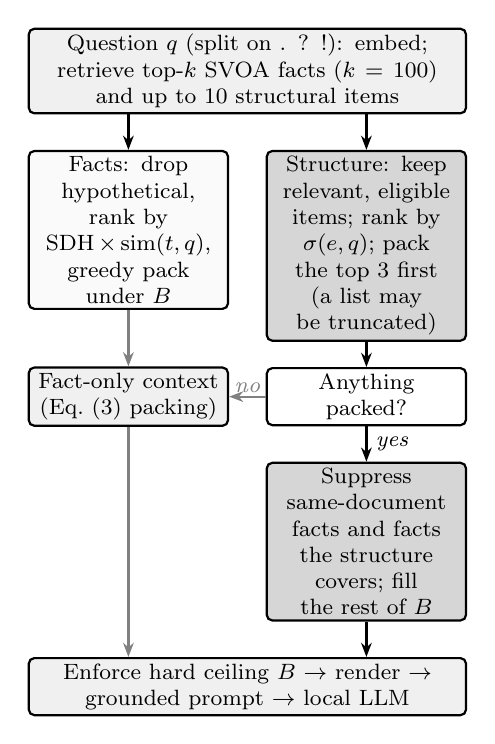
\begin{tikzpicture}[
  font=\fontsize{8}{9.5}\selectfont, >={Stealth[length=1.8mm]}, node distance=3.2mm and 3mm,
  box/.style={draw, thick, rounded corners=2pt, align=center, inner sep=2pt, fill=black!6, text width=#1,
    execute at begin node={\hyphenpenalty=10000\exhyphenpenalty=10000}},
  box/.default=68pt,
  sbox/.style={box=#1, fill=black!16}, sbox/.default=68pt,
  ar/.style={->, thick},
  gar/.style={->, thick, black!50},
  lab/.style={font=\fontsize{8}{9.5}\selectfont\itshape, inner sep=1pt}]
\node[box=154pt] (emb) {Question $q$ (split on . ? !): embed; retrieve top-$k$ SVOA facts ($k=100$) and up to 10 structural items};
\node[box, fill=black!2, below=4.5mm of emb.south west, anchor=north west] (facts)
  {Facts: drop hypothetical, rank by SDH\,$\times$\,sim$(t,q)$, greedy pack under $B$};
\node[sbox, below=4.5mm of emb.south east, anchor=north east] (struct)
  {Structure: keep relevant, eligible items; rank by $\sigma(e,q)$; pack the top 3 first (a list may be truncated)};
\node[box, fill=white, below=of struct] (any) {Anything\\ packed?};
\node[box] (fonly) at (facts |- any) {Fact-only context (Eq.~(3) packing)};
\node[sbox, below=4.5mm of any] (supp)
  {Suppress same-doc\-ument facts and facts the structure covers; fill the rest of $B$};
\node[box=154pt, below=4.5mm of supp.south -| emb.south, anchor=north] (out)
  {Enforce hard ceiling $B$ $\rightarrow$ render $\rightarrow$\\ grounded prompt $\rightarrow$ local LLM};
\draw[ar] (emb.south -| facts.north) -- (facts.north);
\draw[ar] (emb.south -| struct.north) -- (struct.north);
\draw[ar] (struct) -- (any);
\draw[ar] (any) -- node[lab, right=2pt] {yes} (supp);
\draw[gar] (any) -- node[lab, above] {no} (fonly);
\draw[gar] (facts) -- (fonly);
\draw[gar] (fonly.south) -- (out.north -| fonly.south);
\draw[ar] (supp.south) -- (out.north -| supp.south);
\end{tikzpicture}

\caption{Query-time flow: fact packing (left) and guarded structural-priority packing (right) before the hard ceiling and generation.}\label{fig:2}
\end{figure}

\leadin{Stage 0: Hardware profiling.} The profiler reads CPU cores, RAM and GPU memory and selects a token ceiling of 4,096 (RAM $\geq$ 8 GB and VRAM $\geq$ 6 GB), 3,072 (RAM $\geq$ 8 GB and VRAM $\geq$ 2 GB), 2,048 (RAM $\geq$ 16 GB without a qualifying GPU) or 1,024 (other hosts), with a default model per mode (hardware.py). These rules were not evaluated: in the experiments the ceiling was fixed at 2,048 estimated tokens unless Section~\ref{sec:6.4} varies it, and the generator was fixed per experiment. The evaluation host was an AMD Ryzen 9 8945HS laptop with 16 GB RAM and an NVIDIA RTX 4060 Laptop GPU (8 GB VRAM); CPU-only operation, memory use and ingestion and retrieval latency were not measured; generation time is reported in Section~\ref{sec:6.9}.

\leadin{Stage 0.5: Structural retention.}  When the feature flag PRECIS\_\allowbreak{}ENABLE\_\allowbreak{}LIST\_\allowbreak{}EXTRACTION is on, HTML tables and lists are separated from prose; the flag is off by default, so the released application answers with the fact-only configuration (Précis v3 below) unless it is set, and with G when it is. Tables are rendered as compact GitHub-flavoured Markdown and scored per question: 2 for each header matching a question word, 4 for each header matching a requested attribute, 3 for each caption word and 1 for any cell match. A table is selected at a score of at least 2, or if it is a small infobox (three rows or fewer) with a header or caption match, and it is rejected if the question names it as an exclusion. Lists keep their hierarchy, navigation lists are discarded, and tables that duplicate lists are removed.

\leadin{Stages 1–3: Fact layer.} F-coref \cite{r44} replaces pronouns with their referents, a spaCy dependency parse \cite{r45} yields SVOA facts with rule-based negation and modality labels, and the facts are scored with SDH and written to ChromaDB with their modality, adjuncts, attribution, source document and sentence index (Appendix B.1).

\leadin{Stage 4: Query-adaptive packing.}  Multi-part questions are split on sentence punctuation, and up to \textit{k} = 100 candidates per part are retrieved and merged. Hypothetical facts are removed by default; survivors are sorted by (\ref{eq:1}), with modality priority (asserted, attributed, conditional) breaking ties, and added greedily while the running cost stays within \textit{B}. A fact that does not fit is skipped and later, cheaper facts may still be added. In Candidate G, up to ten structural items are retrieved in parallel and handled by (\ref{eq:4}) and the suppression rule of Section~\ref{sec:problem} (Fig.~\ref{fig:2}, right branch). Truncation applies only to a list that does not fit (it is cut at a line boundary if more than 30 tokens remain after the header), and the assembled context is trimmed to the hard ceiling as a last step.

\leadin{Stage 5: Local generation.}  Packed content is inserted into a grounding prompt that tells the model to use only the supplied context, to preserve negation, and not to present attributed, conditional or hypothetical claims as established. The application supports a \textit{standard} and a \textit{concise} answer-formatting template; the controlled experiments below fix the template per condition.

The complete procedure is given as Algorithm 1.

\begin{figure*}[!t]
\noindent \leadin{Algorithm 1:} Précis ingestion and budgeted query answering with guarded structural priority\par\vspace{2pt}
\begin{lstlisting}[basicstyle=\scriptsize\ttfamily,breaklines=true,columns=fullflexible,keepspaces=true,frame=single]
Input : document X, question q, hardware profile H, stores G (facts), S (structure)
Output: answer a, packed context K, estimated tokens used
 1  B     <- CEILING[ MODE(H) ]                     // Stage 0
 2  prose, E <- SplitStructure(X)                    // Stage 0.5 (flag): E = tables, lists
 3  F <- ExtractSVOA( Coref(prose) )                 // Stages 1-2
 4  for each fact t in F, in order do SDH(t) <- aE + bI + gU(t, G u F[<t]) + dA  end for
 5  G <- G u F ;  S <- S u E                         // Stage 3, 384-d cosine index
 6  C <- TopK(G, q, k=100) minus { t : modality(t) = hypothetical }
 7  sort C by ( SDH(t)*sim(t,q), priority(modality(t)) ) descending
 8  P <- greedy pack of C under B                    // Eq. (3)
 9  R <- relevant, eligible structural items of TopK(S, q, 10), ranked by sigma (Eq. (4))
10  Sel <- first 3 of R ; Z <- items of Sel packed first within B (a list may be truncated)
11  if Z is empty then K <- Render(P)                // fact-only fallback
12  else  P' <- { t in P : doc(t) not in doc(Z), and not both s,o of t occur in Z }
13       K <- Z + facts of P' that fit in the remaining budget
14  K <- TrimToCeiling(K, B)
15  a <- LLM( GroundedPrompt( K, q ) )                // Stage 5
16  return a, K, tokens(K)
\end{lstlisting}
\end{figure*}

\section{Results and Discussion}\label{sec:results}

\subsection{Experimental Setup}\label{sec:6.1}

All results come from the authors' harness on the evaluation host of Table~\ref{tab:3}, and the cohorts are analysed separately and never pooled.

Scoring is the same in every cohort. A prediction is correct for exact match if its normalised text equals the gold answer or any alternative answer that MRQA lists, and correct for containment if a normalised answer occurs in it at word boundaries. The rule is implemented once (scripts/scoring.py); re-scoring the prompt experiment, which was first scored against the single gold answer, changed 3 of 800 exact-match and 9 of 800 containment outcomes and left the primary test of Section~\ref{sec:6.6} unchanged. ROUGE-L, MiniLM cosine and BERTScore, and the reference shown to the equivalence judge, use the single gold answer.

\leadin{Inference plan.} Each analysis has one declared status. (a) The original table cohort (Table~\ref{tab:4}) is in-sample, because G was designed on it, and descriptive (unadjusted exact McNemar tests, question-level bootstrap intervals). (b) On the fresh cohort the primary family (exact match; G against D, F2, N\_raw and N\_clean; two-sided exact McNemar, Holm over four contrasts) was fixed in a protocol before any model call. (c) Baseline adequacy (Section~\ref{sec:6.3}) compares G with seven arms by the lower bound of a 99\% question-level bootstrap interval (10,000 resamples); because the 5-point non-inferiority margin was chosen after the fresh-cohort results (and before W, TC and H were run), verdicts are given for margins of 3 to 7 points, with Newcombe paired score intervals and a Bonferroni level for seven comparisons as checks. (d) In the prompt experiment (Section~\ref{sec:6.6}) the primary test is one-sided McNemar for qwen3.5:4b with Précis v3. (e) On the long-document cohort (Section~\ref{sec:6.4}) the primary family (exact match at the 2,048 ceiling; G against N, N\_raw, W, TC and H; non-inferiority at 5 points by 99\% bootstrap intervals; two-sided exact McNemar with Holm) and the margin were fixed before the draw, and G2 was tested on a second, fresh draw under its own protocol (G2 against G, and non-inferiority to TC at 5 points by a 97.5\% interval; Holm over the two). Everything else (the ceiling sweeps, with Holm over their 15 contrasts, the threshold sensitivity, the strata and the 2×2 follow-up) is exploratory. The protocols are author-held files whose SHA-256 hashes and time stamps were written before the model calls; they were neither registered externally nor under version control during the runs, so their order relative to the data cannot be verified independently, and they are called protocol-first below. Clustering is handled by resampling questions (187 distinct questions in the 200 cases of the original cohort, 74 in the 200-sample benchmark, distinct by construction elsewhere). Each case is a single greedy generation; repeating identical contexts changed 3 of 200 exact-match outcomes (Section~\ref{sec:6.5}), the size of the smallest differences reported, so verdicts that rest on one or two cases are within that noise. With 10 to 20\% discordant pairs, 200 paired cases detect about 6 to 9 points at 80\% power (two-sided 5\% level). A non-significant difference is never read as equivalence.

\begin{table*}[!t]
\centering\renewcommand{\arraystretch}{1.15}\footnotesize
\caption{Experimental configuration of the controlled evaluations.}\label{tab:3}
\begin{adjustbox}{max width=\textwidth}
\begin{tabular}{>{\raggedright\arraybackslash}p{0.17\textwidth}>{\raggedright\arraybackslash}p{0.78\textwidth}}
\hline
\textbf{Parameter} & \textbf{Specification} \\
\hline
Data source & MRQA 2019 \cite{r46} version of Natural Questions \cite{r47}, development split; full NQ v1.0 development pages for the long-document cohort \\
Inference & Local Ollama \cite{r41}; qwen2.5-coder:7b \cite{r48} and qwen3.5:4b \cite{r49}; no cloud calls \\
Decoding & Temperature 0.0, top-p 0.9, seed 42, at most 512 generated tokens \\
Context ceiling & 2,048 estimated tokens (word-count proxy, see~(\ref{eq:2})) \\
Additional baselines & W: whole-document Markdown, truncated at the ceiling; TC: table-aware chunks, dense retrieval; H: the same chunks, BM25 + dense with reciprocal rank fusion \cite{r30,r31} \\
Fact store and encoder & Embedded ChromaDB, cosine distance; all-MiniLM-L6-v2 (384-d) \\
Chunked baseline & 512-word chunks, 128-word overlap, top-5 retrieval (used as “Naive RAG” in Section~\ref{sec:6.6}) \\
Metrics & Exact match (EM) and word-boundary containment (gold answer or any MRQA alternative), ROUGE-L \cite{r50}, BERTScore \cite{r51} (deberta-large-mnli \cite{r52}), MiniLM cosine \\
Statistics & Exact McNemar (paired binary), Holm / Bonferroni / Benjamini–Hochberg, question-level bootstrap (10,000 resamples), Newcombe paired score intervals, Wilson intervals \\
Evaluation host & AMD Ryzen 9 8945HS, 16 GB RAM, RTX 4060 Laptop GPU (8 GB VRAM); spaCy 3.8.14, en\_\allowbreak{}core\_\allowbreak{}web\_\allowbreak{}lg 3.8.0 \\
Replay generator and judge & qwen3.5:9b \cite{r53} and gemma4:e4b \cite{r54} (thinking off) on the stored, generator-independent contexts; gemma4:12b \cite{r54} (Ollama) as answer-equivalence judge, temperature 0 \\
\hline
\end{tabular}
\end{adjustbox}
\end{table*}

\subsection{Structural Preservation on Table-Bearing Documents (RQ1)}\label{sec:6.2}

The table-bearing cohort has 200 cases drawn with seed 42 from MRQA Natural Questions development documents whose raw HTML contains a table, unordered-list or ordered-list marker, after excluding 600 historically used identifiers. The 200 cases hold 187 distinct questions (12 questions occur more than once), so the paired tests treat a few repeated questions as independent. The gold answer string occurs in the text of at least one table for 164 of the 200 cases (82\%) and elsewhere in the source document for the other 36 (a string-presence check); cases were selected for table or list markup, not for answers located in a table. The same draw also produced a 100-case prose-only stratum, which was never run. All variants used qwen2.5-coder:7b with greedy decoding, the concise prompt and a 2,048-token ceiling. Predictions for variants A–F were reused unchanged from frozen records, and G was generated live. The variants are: A, a prose baseline (raw document HTML passed through coreference resolution and prose-only SVOA extraction, with no table or list handling and no passage chunking); B, SVOA-decompiled prose, in which the system's own extractor rewrites tables as sentences; C, conservative table retention (distance threshold 2.0); D, table retention alone (threshold 0.0, tables kept as Markdown, no lists or facts); E, an in-memory prototype retaining tables and lists; F, the persistent production pipeline (ChromaDB storage, similarity-dominant ranking, residual context filled with SVOA facts); and G, Candidate G, which adds guarded structural-priority packing.

\begin{table*}[!t]
\centering\renewcommand{\arraystretch}{1.15}\footnotesize
\caption{Structural-preservation ablation on the table-bearing cohort (N = 200). \textit{p}-values are unadjusted two-sided exact McNemar tests.}\label{tab:4}
\begin{adjustbox}{max width=\textwidth}
\begin{tabular}{c>{\raggedright\arraybackslash}p{0.2\textwidth}cc>{\centering\arraybackslash}p{1.5cm}c>{\centering\arraybackslash}p{1.5cm}c}
\hline
\textbf{Var.} & \textbf{Pipeline} & \textbf{Exact match} & \textbf{Containment} & \textbf{G − var. EM (pp)} & \textbf{\textit{p}, EM} & \textbf{G − var. Cont. (pp)} & \textbf{\textit{p}, Cont.} \\
\hline
A & Prose baseline & 64/200 (32.0\%) & 87/200 (43.5\%) & +23.0 & 1.7 × 10\textsuperscript{-9} & +25.0 & 1.5 × 10\textsuperscript{-9} \\
B & SVOA-decompiled prose & 28/200 (14.0\%) & 39/200 (19.5\%) & — & — & — & — \\
C & Table retention, $\theta$ = 2.0 & 61/200 (30.5\%) & 79/200 (39.5\%) & — & — & — & — \\
D & Table retention alone, $\theta$ = 0.0 & 99/200 (49.5\%) & 122/200 (61.0\%) & +5.5 & 0.019 & +7.5 & 0.0015 \\
E & Prototype tables + lists & 108/200 (54.0\%) & 137/200 (68.5\%) & +1.0 & 0.727 & 0.0 & 1.000 \\
F & Persistent production pipeline & 105/200 (52.5\%) & 131/200 (65.5\%) & +2.5 & 0.424 & +3.0 & 0.307 \\
G & Guarded structural priority & 110/200 (55.0\%) & 137/200 (68.5\%) & ref. & ref. & ref. & ref. \\
\hline
\end{tabular}
\end{adjustbox}
\end{table*}

Table~\ref{tab:4} gives the results. Rewriting tables as extracted sentences (B, 14.0\% EM) was the weakest variant and fell below the prose baseline (A, 32.0\%), whereas retaining tables in native form (D) reached 49.5\%; D beat B in 79 cases against 8 (exact McNemar p = 8 × 10\textsuperscript{-16}; question-level 95\% interval +27.3 to +43.9 points). B measures the cost of this extractor's conversion, which has the defects reported in Section~\ref{sec:6.8}, not the cost of every tables-to-text method. Candidate G had the highest exact match (110/200, 55.0\%) and, with E, the highest containment (137/200). Its leads over F (+2.5 points, 15 against 10 discordant pairs, p = 0.42; 95\% interval −2.5 to +7.7) and E (+1.0, p = 0.73) are not distinguishable from zero, and its lead over D (+5.5, p = 0.019) does not survive Holm or Bonferroni correction over the four G contrasts (0.058 and 0.077). Because G was designed on this cohort, these results are descriptive.

\leadin{Fresh cohort.} A second table- or list-bearing cohort was drawn under a protocol-first design: 200 distinct questions from the Natural Questions development file whose documents contain table or list markup, excluding every identifier and question used before (1,425 candidate records, 748 distinct questions; seed 42). Five arms were run with qwen2.5-coder:7b, the concise prompt and the 2,048 ceiling: chunked passage retrieval on the raw document (N\_raw) and on tag-stripped text (N\_clean), table retention alone (D), a reconstruction of F without same-document fact suppression (F2; the frozen F cannot be regenerated by the current code) and G. Exact match was 96/200 (48.0\%) for G, 94 for N\_raw, 89 for F2, 88 for N\_clean and 79 for D. In the primary family G exceeded D (20 against 3 discordant cases, Holm p = 0.002) but not F2 (13 against 6, Holm p = 0.50), N\_raw (11 against 9, p = 0.82) or N\_clean (18 against 10, p = 0.50). The lead over D is confined to the 32 list-only documents, where D has no evidence by construction (G 18 correct, D 0), so it is a mechanism check. On the 168 documents with a table, G, D and N\_raw (and W, TC and H of Section~\ref{sec:6.3}) scored 76 to 79 correct, against 71 for tag-stripped chunks and for F2; native tables beat stripped chunks (D against N\_clean) by 4.8 points (17 against 9, p = 0.17, 95\% interval −1.2 to +10.7), which has the expected sign but is not significant at this size. The large structure effect of Table~\ref{tab:4} is therefore a loss from this conversion, not a gain over cheap structure-keeping alternatives. Taking every cheap structure-keeping baseline (N\_raw, W, TC and H) that was run on a protocol-first cohort, at the 2,048 ceiling and against that cohort's tag-stripped chunks, gives ten comparisons: +3.0 to +5.0 points on the fresh cohort, and −2.5 (N\_raw) to +6.0 (TC) on the two long-document draws; none is significant (smallest p = 0.076). At 1,024 tokens on long pages raw-markup chunks were behind (−10.0 points, p = 0.001), and D, which keeps tables but not lists, was behind on the whole fresh cohort (−4.5). In the exploratory sweeps (Section~\ref{sec:6.4}) H and W against budgeted stripped chunks ranged from −5.5 to +8.5 points, none significant after Holm correction over these ten (smallest unadjusted p = 0.0095). Keeping structure was therefore never shown to beat stripping it at the main ceiling, and keeping raw markup can cost accuracy on long pages.

\leadin{Context size.} Against the authors' own pipelines G's packed context was smaller: 56.2\% fewer estimated tokens than F2 on the fresh cohort (401.8 against 917.9; paired mean difference −516 tokens, 95\% interval −573 to −461) and 53.2\% fewer than F on the original cohort (365.8 against 781.1), or 43 to 46\% fewer model-reported prompt tokens. Against external baselines it is not smaller (Section~\ref{sec:6.3}). The estimate understates native length: native prompt tokens ran at about 1.24 per estimated context token, and at the 2,048 ceiling the full native prompt exceeded 2,048 tokens in 41 F cases and 1 G case.

\subsection{Baseline Adequacy and Efficiency (RQ1)}\label{sec:6.3}

The fresh cohort was re-run with three further arms that do not use the SVOA or SDH code and are cheap to build: W, the whole document converted from HTML to Markdown in document order (tables as Markdown tables, lists as bullets) and truncated at the ceiling; TC, table-aware chunks (tables kept whole or split by rows with the header repeated, lists kept whole, prose grouped to about 128 words) retrieved by dense similarity; and H, the same chunks retrieved by BM25 and dense rankings fused by reciprocal rank fusion. All use the 2,048-token ceiling, at most five chunks, qwen2.5-coder:7b and the concise prompt (protocol and hash in the repository). Table~\ref{tab:5} gives exact match, containment, mean estimated context tokens, exact-match points per 100 tokens, the exact-match difference of G from each arm with its 99\% interval, and the smallest margin, among 3 to 7 points, at which G is non-inferior. The last column gives exact match when the same contexts are answered by a general-purpose generator, qwen3.5:9b, because qwen2.5-coder is a code model.

\begin{table*}[!t]
\centering\renewcommand{\arraystretch}{1.15}\footnotesize
\caption{Baseline adequacy on the fresh table- and list-bearing cohort (N = 200, 2,048-token ceiling, qwen2.5-coder:7b except the last column). N\_raw, N\_clean, D, F2 and G are the earlier records; W, TC and H were run for this table. G − arm is positive when G is ahead. The margin column uses the 99\% bootstrap lower bound; Newcombe paired intervals give the same values except 6 for H.}\label{tab:5}
\begin{adjustbox}{max width=\textwidth}
\begin{tabular}{>{\raggedright\arraybackslash}p{0.2\textwidth}>{\centering\arraybackslash}p{1.0cm}>{\centering\arraybackslash}p{1.0cm}>{\centering\arraybackslash}p{1.0cm}>{\centering\arraybackslash}p{1.0cm}>{\centering\arraybackslash}p{1.25cm}>{\centering\arraybackslash}p{2.6cm}>{\centering\arraybackslash}p{1.8cm}>{\centering\arraybackslash}p{1.5cm}}
\hline
\textbf{Arm} & \textbf{EM /200} & \textbf{Cont. /200} & \textbf{Mean tokens} & \textbf{EM pp per 100 tok} & \textbf{G − arm, EM pp [99\% CI]} & \textbf{Smallest NI margin met (pp)} & \textbf{EM, qwen3.5:9b} \\
\hline
N\_raw (chunks, markup) & 94 & 124 & 503 & 9.3 & +1.0 [-4.5, 7.0] & 5 & 99 \\
N\_clean (chunks, stripped) & 88 & 115 & 280 & 15.7 & +4.0 [-2.5, 11.0] & 3 & 106 \\
W (whole doc, Markdown) & 98 & 129 & 388 & 12.6 & -1.0 [-4.5, 2.5] & 5 & 100 \\
TC (table-aware chunks) & 96 & 126 & 420 & 11.4 & +0.0 [-4.5, 5.0] & 5 & 98 \\
H (hybrid, table-aware) & 98 & 128 & 420 & 11.7 & -1.0 [-6.0, 4.0] & 7 & 98 \\
D (tables only) & 79 & 104 & 351 & 11.3 & +8.5 [3.0, 14.5] & G higher & 84 \\
F2 (F without suppression) & 89 & 120 & 918 & 4.8 & +3.5 [-2.0, 9.5] & 3 & 85 \\
G (guarded priority) & 96 & 127 & 402 & 11.9 & reference & — & 98 \\
\hline
\end{tabular}
\end{adjustbox}
\end{table*}

G was not distinguishable from any structure-keeping baseline: its exact-match differences from N\_raw, W, TC and H lay between −1.0 and +1.0 points. Whether this counts as non-inferiority depends on a margin chosen after the fresh-cohort results were known. At 5 points G is non-inferior to N\_raw, N\_clean, W, TC and F2 but not to H; at 4 points only N\_clean and F2 remain; and at a Bonferroni level for seven comparisons (99.3\%) the Newcombe lower bounds against N\_raw and TC (−5.1) cross the 5-point margin and that against W (−4.95) just meets it. The verdicts against N\_raw, W and TC therefore rest on one or two cases, and non-inferiority to TC with its absence for H is not itself a supported difference. Efficiency does not favour G either: per 100 estimated tokens the order was N\_clean (15.7), W (12.6), G (11.9), H (11.7), TC (11.4), D (11.3), N\_raw (9.3) and F2 (4.8), and G's context was 13.5 tokens larger than W's (paired 95\% interval +1.0 to +29.9), about 18 tokens smaller than TC's and H's, 102 smaller than N\_raw's and 122 larger than N\_clean's. These counts cover the context only: G also needs coreference resolution, parsing and SDH scoring at ingestion, whereas W and TC need only an HTML conversion.

Retrieval and packing make no model call, so each arm's context is the same whichever generator answers it, and answering the stored contexts with another generator is equivalent to running the whole pipeline with it. With qwen3.5:9b, G was +7.0 points above D (p = 0.004) and +6.5 above F2 (p = 0.004), and was not distinguishable from N\_raw (−0.5, p = 1.00), N\_clean (−4.0, p = 0.18), W (−1.0), TC (+0.0) or H (+0.0). A third generator from another family, gemma4:e4b (exploratory, protocol-first), had lower exact match throughout (78 for G) and put G in the same position relative to the structure-keeping baselines: not distinguishable from N\_raw (+1.0), N\_clean (+1.0), W (−2.0, p = 0.22), TC (−2.5, p = 0.27) or H (0.0), and above D (+6.5, p = 0.002); only its lead over F2 was not reproduced (−1.5, p = 0.58). The position of G relative to the baselines therefore does not depend on the code-specialised generator.

\subsection{Where the Ceiling Binds (RQ1)}\label{sec:6.4}

At the 2,048 ceiling the budget barely binds on this data: G's largest context was 1,163 estimated tokens, and in the 200-sample benchmark of Section~\ref{sec:6.7} 186 of 200 passages fit in one 512-word chunk. MRQA documents are short (the longest in the 12,836-record development file has 800 words), which is consistent with the release truncating long pages. Two exploratory experiments therefore make the ceiling bind, and a third, protocol-first cohort uses full pages (below). First, the same single documents were run with ceilings of 256, 512 and 1,024 estimated tokens, comparing G with budgeted chunks (the N arm, tag-stripped 512-word chunks cut at the ceiling), H and W. Second, each question was placed in a five-document corpus (the relevant document and four random distractors, in shuffled order; mean 1,523 estimated tokens) with ceilings of 1,024 and 2,048; G ingested all five documents, the chunked arms treated the concatenation as one text, and W truncated it. Table~\ref{tab:6} gives exact match and, in brackets, the number of the 200 contexts that contain an answer string; Fig.~\ref{fig:3} plots the exact-match values.

\begin{table*}[!t]
\centering\renewcommand{\arraystretch}{1.15}\footnotesize
\caption{Exploratory ceiling sweeps (N = 200): exact match, with the number of contexts containing an answer string in brackets. qwen2.5-coder:7b, concise prompt.}\label{tab:6}
\begin{adjustbox}{max width=\textwidth}
\begin{tabular}{>{\raggedright\arraybackslash}p{0.24\textwidth}>{\centering\arraybackslash}p{1.6cm}>{\centering\arraybackslash}p{1.6cm}>{\centering\arraybackslash}p{1.6cm}>{\centering\arraybackslash}p{1.6cm}>{\centering\arraybackslash}p{2.4cm}}
\hline
\textbf{Setting, ceiling (est. tokens)} & \textbf{G} & \textbf{N (chunks)} & \textbf{H (hybrid)} & \textbf{W (truncated)} & \textbf{Mean tokens, G / N} \\
\hline
Single document, 256 & 67 (150) & 89 (191) & 78 (168) & 87 (181) & 194 / 181 \\
Single document, 512 & 91 (189) & 87 (199) & 91 (184) & 98 (194) & 292 / 242 \\
Single document, 1,024 & 96 (197) & 87 (199) & 97 (197) & 98 (199) & 384 / 276 \\
Five-document corpus, 1,024 & 90 (195) & 74 (181) & 91 (189) & 71 (163) & 923 / 1,000 \\
Five-document corpus, 2,048 & 86 (196) & 81 (198) & 92 (193) & 91 (196) & 1,654 / 1,440 \\
\hline
\end{tabular}
\end{adjustbox}
\end{table*}

\begin{figure*}[!t]
\centering
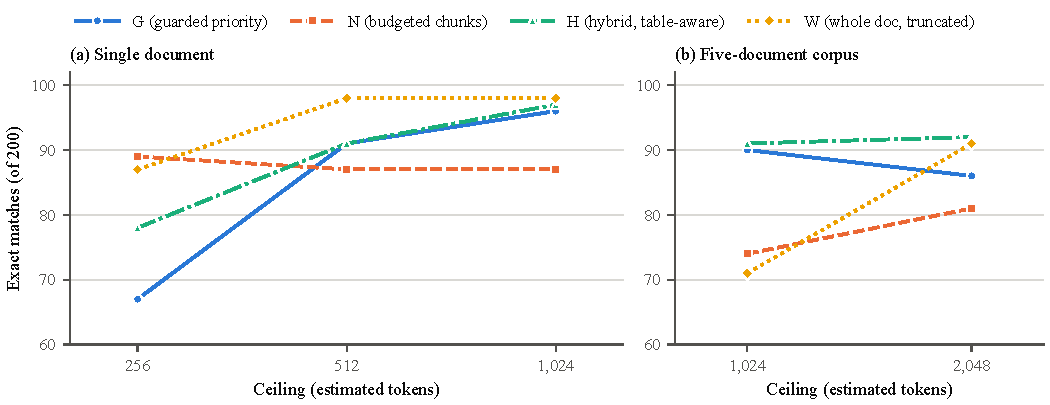
\includegraphics[width=\textwidth]{figure_3_ceiling_sweep.pdf}
\caption{Exploratory ceiling sweeps of Table~\ref{tab:6} (N = 200, qwen2.5-coder:7b, concise prompt): exact match against the ceiling for G, budgeted tag-stripped chunks (N), hybrid table-aware retrieval (H) and truncated whole-document Markdown (W), on (a) single documents and (b) five-document corpora.}\label{fig:3}
\end{figure*}

With a single document and a 256-token ceiling the budget binds and G loses: exact match 67 against 89 for chunks (−11.0 points, 11 against 33 discordant cases, Holm p = 0.018 over the 15 contrasts of Table~\ref{tab:6}) and 87 for W (Holm p = 0.008), with only 150 of 200 G contexts still containing an answer string against 191 for chunks. The likely cause is that G packs a structural element first and truncates one that does not fit, which was not examined separately; row-level truncation with repeated headers, as in TC, is the obvious remedy. At 512 and 1,024 tokens G was level with chunks and H. In five-document corpora at a 1,024 ceiling G was ahead of budgeted chunks (90 against 74; unadjusted p = 0.014, Holm 0.17) and of truncated Markdown (71; Holm 0.056) and level with H (91); at 2,048 tokens G (86) was not distinguishable from chunks (81), H (92) or W (91). The curves are not monotone, which is consistent with noise of several cases. The sweeps show a clear disadvantage of G at a very small ceiling and no advantage over hybrid table-aware retrieval in any setting.

\leadin{What the ceiling bounds.} B applies to the word-count estimate of (\ref{eq:2}), not to the generator's tokens; the generator was given a context window large enough for every prompt, so nothing was truncated by the model server.

\leadin{Long documents.} Because MRQA cuts every page to at most 800 words, a third cohort was drawn under a protocol fixed before the draw, with the primary family and a 5-point non-inferiority margin stated in advance: 200 questions from the full development pages of Natural Questions v1.0 \cite{r47} whose page contains a table and at least 3,000 words of text, excluding every question used before (902 eligible questions among the 3,357 examples of the first three of the seven development shards, as the protocol fixed; seed 42). The median page had 7,093 words (9,625 estimated tokens), so the 2,048 ceiling covered about a fifth of it; the answer lay inside a table for 33 questions and beyond the first 1,575 words, which whole-document truncation can reach, for 57. Arms G, N, N\_raw, W, TC and H were run as before with qwen2.5-coder:7b and the concise prompt at ceilings of 2,048 (primary) and 1,024 estimated tokens. Table~\ref{tab:7} gives the results. A GPU out-of-memory error stopped the run once; a retry was added, the completed cases were kept and none was regenerated (as for the other interrupted runs, logged in the repository).

\begin{table*}[!t]
\centering\renewcommand{\arraystretch}{1.15}\footnotesize
\caption{Long-document cohort (N = 200 full Natural Questions pages, median 7,093 words): exact match, contexts containing an answer string and mean estimated tokens at the 2,048 ceiling, the exact-match difference of G from each arm with its 99\% bootstrap interval and Holm-adjusted McNemar p, and exact match at 1,024. qwen2.5-coder:7b, concise prompt.}\label{tab:7}
\begin{adjustbox}{max width=\textwidth}
\begin{tabular}{>{\raggedright\arraybackslash}p{0.2\textwidth}>{\centering\arraybackslash}p{1.4cm}>{\centering\arraybackslash}p{1.4cm}>{\centering\arraybackslash}p{1.4cm}>{\centering\arraybackslash}p{2.8cm}>{\centering\arraybackslash}p{1.2cm}>{\centering\arraybackslash}p{1.4cm}}
\hline
\textbf{Arm (long documents)} & \textbf{EM /200 at 2,048} & \textbf{Answer in context} & \textbf{Mean tokens} & \textbf{G − arm, EM pp [99\% CI]} & \textbf{Holm p} & \textbf{EM /200 at 1,024} \\
\hline
G (guarded priority) & 44 & 84 & 1,049 & reference & — & 43 \\
N (chunks, stripped) & 71 & 172 & 2,048 & −13.5 [−23.0, −4.0] & 0.001 & 75 \\
N\_raw (chunks, markup) & 66 & 140 & 2,048 & −11.0 [−20.0, −2.5] & 0.002 & 55 \\
W (whole doc, truncated) & 75 & 168 & 2,048 & −15.5 [−24.5, −6.5] & < 0.001 & 78 \\
TC (table-aware chunks) & 83 & 158 & 989 & −19.5 [−28.5, −10.5] & < 0.001 & 79 \\
H (hybrid, table-aware) & 76 & 152 & 1,141 & −16.0 [−25.0, −7.0] & < 0.001 & 76 \\
\hline
\end{tabular}
\end{adjustbox}
\end{table*}

When the ceiling bound on long pages, G was the worst arm: 44 of 200 exact matches against 66 to 83 for the five baselines, 11.0 to 19.5 points behind each of them (Holm p $\leq$ 0.002), so non-inferiority failed against all five at the pre-specified margin. At 1,024 the picture was the same (43 against 55 to 79), except that the gap to raw-markup chunks was not significant (−6.0 points, p = 0.10). Table-aware chunks were best (83 at 2,048, with a smaller context than G's). The loss arose before generation: an answer string was in only 84 of G's 200 contexts, against 140 to 172 for the baselines, and G was behind even on the 33 questions whose answer lay in a table (7 correct against 9 to 14). Fig.~\ref{fig:4} sets these differences beside those of the fresh cohort (Table~\ref{tab:5}): there every interval except that against D includes zero, here every interval lies below zero.

\begin{figure*}[!t]
\centering
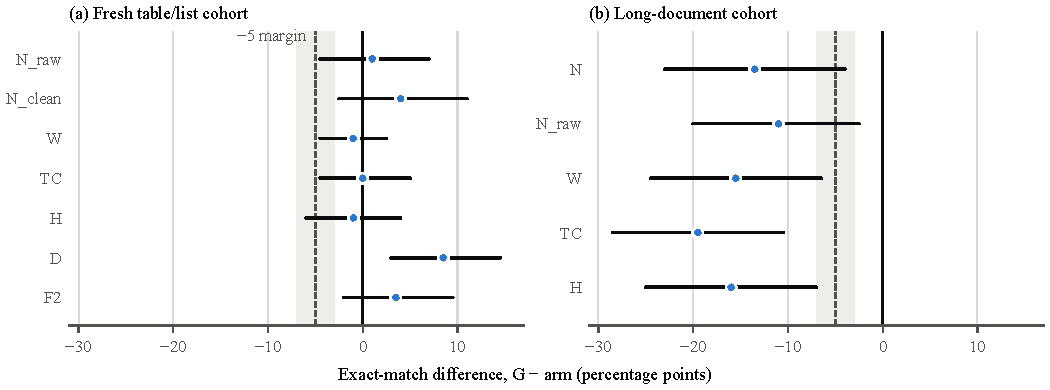
\includegraphics[width=\textwidth]{figure_4_forest.pdf}
\caption{Exact-match difference of G from each arm (percentage points, positive when G is ahead) with its 99\% question-level bootstrap interval, on (a) the fresh table- and list-bearing cohort (Table~\ref{tab:5}) and (b) the long-document cohort at the 2,048 ceiling (Table~\ref{tab:7}). The dashed line marks the 5-point non-inferiority margin and the shaded band the 3 to 7 points over which the fresh-cohort margin was varied.}\label{fig:4}
\end{figure*}

\leadin{Why G fails on full pages.} A descriptive look at G's contexts, made after the results were known, shows the mechanism. None of G's 200 contexts contained a prose fact: on a single document, packing any table or list suppresses every fact of that document (Section~\ref{sec:problem}), and full pages offer many lists. 82 contexts held lists only, and 107 contained reference-list, category or media-link text that the navigation filter, designed on MRQA's extracts, did not remove; G also left about half of the budget unused (1,049 estimated tokens on average). Same-document suppression and unfiltered reference lists, rather than the order of packing as such, are the likely reasons (a reading made after the results) that G is unsuitable for long single documents, and table-aware chunking keeps the benefit of native tables without that failure. The replays through other generators that the protocol listed as exploratory were not run, because the deficit lies in what the contexts contain, which does not depend on the generator.

\leadin{Repair on a fresh draw.} The diagnostic points to two changes, which were tested on questions not used to design them, under a protocol written before a second draw of 200 eligible full pages (none shared with the first; seed 43). The repaired rule G2 suppresses only facts whose subject and object both occur in the packed structural text, not every fact of the page, and skips a structural candidate when at least 30\% of its lines are references or media and external links. On this draw G2 had 67 exact matches against 35 for G (+16.0 points, 38 against 6 discordant cases, Holm p < 0.001, 95\% interval +10.0 to +22.5) and was non-inferior to table-aware chunks at the 5-point margin (63; +2.0 points, 97.5\% interval −4.5 to +9.0); it was level with whole-document Markdown (69; −1.0, p = 0.88) and stripped chunks (61; +3.0, p = 0.45). Every G2 context contained prose facts (none of G's did), an answer string reached 158 of its contexts against 70 for G, and G2 used nearly the whole budget (1,958 estimated tokens on average, against 939 for table-aware chunks, so its parity comes at about twice their context). Table-aware chunks scored 63 on this draw against 83 on the first, so differences between draws are as large as the margin. G2 was designed after the first long-document results and is tested on one further draw from the same source, so it is a repaired variant, not a separately tuned method; it still packs structure first, its two changes were not tested separately, and it is implemented in the experiment script (scripts/run\_\allowbreak{}long\_\allowbreak{}doc\_\allowbreak{}fixed\_\allowbreak{}g.py), not yet in the released pipeline.

\subsection{Threshold Sensitivity of Candidate G}\label{sec:6.5}

The thresholds of (\ref{eq:4}) and the cap of three elements were set on the original cohort. Perturbing each in turn on the fresh cohort (relevance 0.20 and 0.30, keyword-assisted 0.10 and 0.20, eligibility 0.30 and 0.50, cap two and four) changed 0 to 8 of 200 contexts and moved exact match by at most 1 point from the rerun of G (95 correct; the stored G has 96, and the rerun differed from it in 3 of 200 outcomes on identical contexts, which is the decoding noise of the local server at temperature 0). Because so few contexts change, this shows how rarely the cohort exercises the thresholds, not that they carry over to other data.

\subsection{Answer Format and Abstention Policy (RQ2)}\label{sec:6.6}

The main prompt experiment used 100 new question–document pairs from the same MRQA source, selected deterministically from an eligible pool of 3,904 by sorting SHA-256 hashes of normalised questions after removing overlaps with earlier cohorts. It crossed two generators (qwen2.5-coder:7b and qwen3.5:4b), two retrieval conditions (the chunked baseline, here “Naive RAG”, and Précis v3, the fact-only pipeline without the structural packing of G) and two prompts (standard and concise), giving 800 evaluations on contexts cached once per question and condition and checked by SHA-256 parity. Hypotheses, guardrails and tests were written into protocol files time-stamped before the first model output; the guardrails were fixed after an earlier exploratory prompt comparison (on 101 and 100 other samples, not counted as evidence) had shown 48\% containment. Runs used Ollama 0.35.1, Q4\_K\_M quantisation and the templates of Appendix A. The primary hypothesis was that the concise prompt raises Précis exact match for qwen3.5:4b (one-sided exact McNemar, $\alpha$ = 0.05), with guardrails of a containment change of at least −0.25 and concise containment of at least 0.40; three secondary prompt effects used Holm-corrected one-sided tests.

\begin{table*}[!t]
\centering\renewcommand{\arraystretch}{1.15}\footnotesize
\caption{Standard-to-concise prompt outcomes in the 2×2×2 prompt experiment (N = 100 per cell; EM in correct answers out of 100). EM and containment use the gold answer or any MRQA alternative; ROUGE-L, MiniLM and BERTScore use the single gold answer.}\label{tab:8}
\begin{adjustbox}{max width=\textwidth}
\begin{tabular}{>{\raggedright\arraybackslash}p{0.22\textwidth}>{\centering\arraybackslash}p{1.7cm}>{\centering\arraybackslash}p{1.7cm}>{\centering\arraybackslash}p{1.7cm}>{\centering\arraybackslash}p{1.7cm}>{\centering\arraybackslash}p{1.7cm}>{\centering\arraybackslash}p{1.7cm}}
\hline
\textbf{Model / retrieval} & \textbf{EM (std $\rightarrow$ conc.)} & \textbf{Containment} & \textbf{ROUGE-L} & \textbf{MiniLM} & \textbf{BERTScore} & \textbf{Mean tokens} \\
\hline
qwen2.5-coder:7b / Naive RAG & 21 $\rightarrow$ 45 & 0.68 $\rightarrow$ 0.51 & 0.487 $\rightarrow$ 0.566 & 0.616 $\rightarrow$ 0.668 & 0.668 $\rightarrow$ 0.703 & 21.0 $\rightarrow$ 12.2 \\
qwen2.5-coder:7b / Précis v3 & 18 $\rightarrow$ 35 & 0.53 $\rightarrow$ 0.41 & 0.416 $\rightarrow$ 0.445 & 0.565 $\rightarrow$ 0.553 & 0.632 $\rightarrow$ 0.635 & 20.7 $\rightarrow$ 7.4 \\
qwen3.5:4b / Naive RAG & 11 $\rightarrow$ 51 & 0.75 $\rightarrow$ 0.66 & 0.384 $\rightarrow$ 0.684 & 0.560 $\rightarrow$ 0.791 & 0.587 $\rightarrow$ 0.784 & 36.3 $\rightarrow$ 10.3 \\
qwen3.5:4b / Précis v3 & 6 $\rightarrow$ 43 & 0.61 $\rightarrow$ 0.53 & 0.277 $\rightarrow$ 0.604 & 0.491 $\rightarrow$ 0.732 & 0.535 $\rightarrow$ 0.747 & 40.8 $\rightarrow$ 9.9 \\
\hline
\end{tabular}
\end{adjustbox}
\end{table*}

The primary hypothesis was supported: for qwen3.5:4b with Précis v3 exact match rose from 6/100 to 43/100 (37 concise-only against 0 standard-only correct answers; one-sided p = 7.3 × 10\textsuperscript{-12}, identical under single-gold and alias scoring), and containment moved from 0.61 to 0.53, within both guardrails. The three secondary effects were also significant after Holm correction (11 to 51, 18 to 35 and 21 to 45 correct). Containment fell in all four conditions. A gain this large under strict matching is expected when one prompt asks for a bare span \cite{r33,r35}; the follow-up below asks what it consists of.

The retrieval-by-prompt interaction was −0.03 (95\% interval −0.13 to +0.07) for qwen3.5:4b and −0.07 (−0.15 to +0.01) for qwen2.5-coder:7b, so the prompt effect is not shown to differ between retrieval methods. The chunked baseline was numerically ahead of Précis v3, the fact-only configuration, in exact match and in containment in all four model–prompt cells of Table~\ref{tab:8} (for example 51 against 43 correct for qwen3.5:4b under the concise prompt), in the same direction as the benchmark of Section~\ref{sec:6.7}; in exploratory paired tests it was ahead in containment in all four model–prompt strata (unadjusted p = 0.004 to 0.052), but after Holm correction over the eight tests only one difference remains below 0.05. Context coverage accounts for part of the gap: an answer string occurred in all 100 chunked contexts but in only 79 of the 100 fact-only contexts, so the fact layer lost the answer before generation in 21 cases.

\leadin{Separating format from abstention.} The concise prompt differs from the standard one in its answer-format instructions (a short span instead of a sentence) and in its abstention line (output “Insufficient information” instead of saying so explicitly). In a blinded 30-question pilot error audit (60 outputs labelled by one author and one language-model rater; $\kappa$ = 0.70 on merged labels), the concise prompt corrected 12 answers and degraded none; 7 corrections unwrapped a correct entity from a sentence and 5 replaced an abstention. An exploratory follow-up crossed the two factors on the same 100 cached contexts by adding two prompts, each built by swapping only the abstention line (Appendix A): the concise prompt with the standard abstention line (short + explicit) and the standard prompt with the “Insufficient information” line (sentence + token). Table~\ref{tab:9} gives, per cell, exact match, outputs judged equivalent to the gold answer by a local model (gemma4:12b, fixed rubric, temperature 0) and abstaining outputs.

\begin{table*}[!t]
\centering\renewcommand{\arraystretch}{1.15}\footnotesize
\caption{The 2×2 follow-up (N = 100 per cell): exact match / outputs judged equivalent to the gold answer / abstaining outputs. The judge agreed with two human labellers (authors, labelling blind) on 92\% and 97\% of the outputs each could label (Section~\ref{sec:6.6}).}\label{tab:9}
\begin{adjustbox}{max width=\textwidth}
\begin{tabular}{>{\raggedright\arraybackslash}p{0.22\textwidth}>{\centering\arraybackslash}p{2.6cm}>{\centering\arraybackslash}p{2.6cm}>{\centering\arraybackslash}p{2.6cm}>{\centering\arraybackslash}p{2.6cm}}
\hline
\textbf{Model / retrieval} & \textbf{Sentence + explicit (standard)} & \textbf{Sentence + token} & \textbf{Short + explicit} & \textbf{Short + token (concise)} \\
\hline
qwen2.5-coder:7b / Naive RAG & 21 / 84 / 2 & 24 / 56 / 36 & 55 / 79 / 4 & 45 / 64 / 22 \\
qwen2.5-coder:7b / Précis v3 & 18 / 73 / 9 & 10 / 32 / 60 & 43 / 73 / 6 & 35 / 56 / 34 \\
qwen3.5:4b / Naive RAG & 11 / 77 / 17 & 18 / 74 / 19 & 51 / 81 / 3 & 51 / 78 / 9 \\
qwen3.5:4b / Précis v3 & 6 / 56 / 30 & 17 / 59 / 30 & 43 / 70 / 8 & 43 / 67 / 14 \\
\hline
\end{tabular}
\end{adjustbox}
\end{table*}

Averaged over the abstention wording, the short-span format raised exact match by 25.0 to 36.5 points in the four model–retrieval combinations (95\% intervals all above +18), so the large exact-match effect of the concise prompt is mainly a format effect. The abstention wording is a separate factor whose effect depends on the generator and the format. For qwen2.5-coder the “Insufficient information” line raised abstention (from 2 to 36 sentence outputs with Naive RAG and from 9 to 60 with Précis v3), lowered judged-equivalent answers by 21.5 and 29.0 points on average, and lowered exact match in the short format (55 to 45 and 43 to 35; p = 0.006 and 0.021). These abstentions were mostly false: every abstention on a chunked context, and 46 of the 60 sentence-format abstentions on Précis v3 contexts, came from a context that contained an answer string. For qwen3.5:4b it left judged-equivalent answers almost unchanged (−3.0 and 0.0 points) and raised exact match in the sentence format (11 to 18 and 6 to 17; p = 0.016 and 0.001) but not in the short format, where both cells were unchanged; the format-by-abstention interaction for exact match was −11.0 points (95\% interval −18 to −5) for qwen3.5:4b with Précis v3 and −13.0 (−22 to −4) for qwen2.5-coder with Naive RAG. The concise prompt of the main experiment therefore combines a format instruction that changes strict-match scores with an abstention instruction that, for the code-specialised generator, causes abstentions on answerable contexts.

\leadin{Does the format effect survive an equivalence measure?} Mostly not. Averaged over the abstention wording, the format effect on judged-equivalent answers was +1.5 and +4.0 points with Naive RAG (intervals including zero) and +12.0 and +11.0 with Précis v3 (95\% intervals +6.5 to +18.0 and +3.5 to +18.5), so a short answer helped the judged score mainly on fact contexts, whose sentence fragments a sentence answer tends to restate. The headline cell, qwen3.5:4b with Précis v3, moved from 6 to 43 under exact match but from 56 to 67 under the judge. Exact match mostly measures whether an answer is a bare span, and many sentence answers of the standard prompt are equivalent to the gold answer. The retrieval ranking is the same under both measures: the chunked baseline was ahead of Précis v3 in all eight cells under exact match and by 6 to 24 judged-equivalent answers. The judge was checked by one author, who labelled 100 outputs sampled equally from its CORRECT and INCORRECT verdicts without seeing the verdict; 10 marked hard to tell were excluded. On the remaining 90 the two agreed on 83 (92.2\%, Wilson 95\% interval 85–96\%; Cohen's $\kappa$ = 0.84, which the verdict-balanced sample pushes upwards; 92.6\% when the two verdicts are weighted by their frequency among the 1,600 outputs), on 46 of 49 sentence-format and 37 of 41 short-format outputs, so agreement does not differ visibly between the formats being compared, which is where a verbosity bias of the judge \cite{r38} would show. The judge saw the single gold answer whereas exact match accepts MRQA alternatives, which can only make the judge stricter. A second author, who saw neither the first labels nor the verdicts, labelled the same 100 outputs (14 marked hard to tell): the judge agreed with this labeller on 83 of 86 (96.5\%, Wilson 95\% interval 90–99\%; $\kappa$ = 0.93; 97.6\% weighted), and the two labellers agreed on all 76 outputs that both labelled. With two labellers and at most 90 scored outputs each, the judged counts are a supporting measure, and the conclusions about format rest on the direction of the differences, not their size.

\subsection{Information Loss across Pipeline Stages (RQ3)}\label{sec:6.7}

\leadin{Single-passage benchmark.} On a 200-sample development benchmark of short passages (74 distinct questions; 512-word chunks with 128-word overlap, standard prompt, qwen2.5-coder:7b, 2,048 ceiling), chunked retrieval was numerically ahead of the fact-only Précis v3: 57 against 38 exact matches (26 against 7 discordant pairs; question-level 95\% interval for the difference −0.5 to +19.5 points) and 159 against 141 containment. 186 of the 200 passages fit in one chunk, so this setting tests extraction rather than packing, and it does not bear on the table cohorts.

The extraction rules were revised over successive versions (v1, v1.5, v2 and v3) after inspecting failures on this split, raising answer coverage (the answer string in some extracted fact) from 68.5\% (v1) to 88.5\% (v3) and exact match from 14.5\% to 19.0\%; these are in-sample engineering results. Under one procedure without coreference, the current extractor covered 91.0\% of these development documents and 86.6\% of 1,000 held-out documents from the same file (95\% interval 84.4–88.7\%), so the level of coverage, though not the size of the improvement, carries over.

Tracing the answer string through the v3 pipeline gave 200/200 in the source passages, 177/200 in the extracted facts and 177/177 in both the retrieved candidates and the packed context, so in this setting the loss arose at extraction (23 cases) and after packing. Of the 177 covered cases, 141 outputs contained an answer string and 38 were exact matches, so at least 36 covered cases were lost at generation and 103 between containment and exact match. The 177/177 figures are conditional on extraction, and an answer string in a context shows that the answer was available, not that it was used.

The same trace on the table cohort is where retrieval and packing could lose evidence. Table~\ref{tab:10} follows the fresh cohort from the document to the context and to the answer. At the 2,048 ceiling the answer string was in the context in 197 of 200 cases for G and in 198 to 199 for the chunked, Markdown and F2 arms (168 for D, which has no evidence for the 32 list-only documents by construction), so the answer string survived retrieval and packing in nearly every context, and the remaining loss was at generation (abstentions and wrong answers) and at exact matching; 37 of G's 38 abstentions came from a context that held an answer string. The situation changes when the ceiling binds: at 256 estimated tokens the answer string was in only 150 of G's 200 contexts against 191 for chunks (Table~\ref{tab:6}), and that is where packing, not generation, decides the outcome. On full pages the same holds at 2,048: an answer string reached 84 of G's contexts against 140 to 172 for the other arms (Table~\ref{tab:7}).

\begin{table*}[!t]
\centering\renewcommand{\arraystretch}{1.15}\footnotesize
\caption{Stage loss on the fresh table- and list-bearing cohort (N = 200, 2,048-token ceiling, qwen2.5-coder:7b). Rows after the first column count cases whose context contains the answer string; “Abstained” and “Wrong answer” partition those contexts' outputs that do not contain the answer.}\label{tab:10}
\begin{adjustbox}{max width=\textwidth}
\begin{tabular}{l>{\centering\arraybackslash}p{1.9cm}>{\centering\arraybackslash}p{1.9cm}>{\centering\arraybackslash}p{1.9cm}>{\centering\arraybackslash}p{1.9cm}>{\centering\arraybackslash}p{1.9cm}>{\centering\arraybackslash}p{1.9cm}}
\hline
\textbf{Arm} & \textbf{Answer in context} & \textbf{Output contains answer} & \textbf{Exact match} & \textbf{Contains, not exact} & \textbf{Abstained} & \textbf{Wrong answer} \\
\hline
N\_raw & 199 & 124 & 94 & 30 & 32 & 43 \\
N\_clean & 199 & 115 & 88 & 27 & 37 & 47 \\
D & 168 & 104 & 79 & 25 & 33 & 31 \\
F2 & 198 & 120 & 89 & 31 & 38 & 40 \\
G & 197 & 127 & 96 & 31 & 37 & 33 \\
\hline
\end{tabular}
\end{adjustbox}
\end{table*}

\subsection{The Fact Layer: an Extractor Audit}\label{sec:6.8}

No experiment above isolates the SVOA fact layer's contribution to G. In the 200 contexts of G on the original cohort only 111 facts were packed in total, none with a negation marker, so in these cohorts it contributes little to what G packs; where it formed the whole context (Précis v3, Sections~\ref{sec:6.6} and \ref{sec:6.7}) it was behind plain chunks. What can be said is how accurate its labels are. Two human annotators, working independently, labelled, from 700 randomly drawn development documents (7,824 extracted facts, of which 184, 2.4\%, were flagged negated), 400 facts sampled at random within strata (seed 42) to include 130 of the 184 negated, 120 non-asserted and 150 asserted ones, and 200 sentences (100 containing a negation cue, 60 a hedge, attribution or condition cue, and 40 neither). For each fact they judged, with the stored labels visible, whether the stored negation flag and the stored modality were right; for each sentence, blind to the extractor, whether its main claim is negated and which of four modalities it carries (asserted, attributed, conditional, hypothetical). A language model was used only to reword the free-text notes that accompany one annotator's labels. 12 facts and 7 sentences that one annotator marked ambiguous or too thin to judge were excluded, leaving 388 facts and 193 sentences. Agreement between the annotators was $\kappa$ = 0.86 for stored polarity, 0.50 for stored modality, 0.80 for sentence negation and 0.71 for sentence modality (prevalence-adjusted agreement, PABAK, 0.92, 0.81, 0.92 and 0.85). Table~\ref{tab:11} reports precision per stored class and recall at sentence level.

\begin{table*}[!t]
\centering\renewcommand{\arraystretch}{1.15}\footnotesize
\caption{Extractor audit: precision of the stored negation flag and modality per stored class (facts), and negation and non-asserted-modality recall and precision at sentence level, per annotator and where both agree. Counts in brackets; n for sentence rows lists A / B / agreed. The sample is enriched for negated and non-asserted facts and for cue-bearing sentences, so precision is per class, not overall, and sentence precision is lowered by the enrichment.}\label{tab:11}
\begin{adjustbox}{max width=\textwidth}
\begin{tabular}{>{\raggedright\arraybackslash}p{0.3\textwidth}>{\centering\arraybackslash}p{1.6cm}>{\centering\arraybackslash}p{2.4cm}>{\centering\arraybackslash}p{2.4cm}>{\centering\arraybackslash}p{2.4cm}}
\hline
\textbf{Measure} & \textbf{n} & \textbf{Annotator A} & \textbf{Annotator B} & \textbf{A and B agree} \\
\hline
Polarity correct, stored negated & 123 & 43.9\% (54/123) & 44.7\% (55/123) & 43.5\% (47/108) \\
Polarity correct, stored not negated & 265 & 99.6\% (264/265) & 100.0\% (265/265) & 100.0\% (264/264) \\
Modality correct, stored asserted & 255 & 93.3\% (238/255) & 92.5\% (236/255) & 96.6\% (227/235) \\
Modality correct, stored attributed & 89 & 78.7\% (70/89) & 71.9\% (64/89) & 80.0\% (60/75) \\
Modality correct, stored conditional & 12 & 100.0\% (12/12) & 100.0\% (12/12) & 100.0\% (12/12) \\
Modality correct, stored hypothetical & 32 & 93.8\% (30/32) & 96.9\% (31/32) & 100.0\% (29/29) \\
Sentence negation, recall & 21 / 25 / 19 & 81.0\% (17/21) & 80.0\% (20/25) & 78.9\% (15/19) \\
Sentence negation, precision & 56 / 56 / 49 & 30.4\% (17/56) & 35.7\% (20/56) & 30.6\% (15/49) \\
Sentence non-asserted modality, recall & 46 / 41 / 29 & 71.7\% (33/46) & 70.7\% (29/41) & 72.4\% (21/29) \\
Sentence non-asserted modality, precision & 46 / 46 / 33 & 71.7\% (33/46) & 63.0\% (29/46) & 63.6\% (21/33) \\
\hline
\end{tabular}
\end{adjustbox}
\end{table*}

The negation flag was wrong for more than half of the facts it marked negated: 43.9\% of 123 stored-negated facts had correct polarity by annotator A (Wilson 95\% interval 35–53\%), 44.7\% by B and 43.5\% where both agree, against 99.6\% of non-negated facts, and in 55 of the 69 wrong cases (80\%) no negation cue occurs in the fact's own subject, verb or object (an automatic check), which indicates negation attached to a fact from another clause of the same sentence, not a missed cue. Sentence-level recall of negation was about 80\% (81.0\% by A, 95\% interval 60–92\%, on only 21 negated sentences), but sentence-level precision was about 30\% in this cue-enriched sample, which is consistent with the same over-attachment. Modality labels were more accurate: asserted facts were correct 93.3\% of the time by A (92.5\% by B), attributed facts 78.7\% (71.9\%), and the few conditional and hypothetical facts were almost all correct, but annotators disagreed more on whether a stored modality was right ($\kappa$ = 0.50), and A marked 38 stored modalities wrong, 3 of them without naming a different class; among the other 35 the most frequent corrections were attributed facts that were really asserted (17) and the reverse (7). The audit supports a limited claim: the fact layer's modality labels are mostly right for asserted facts, but its negation flag, which the system's grounding prompt asks the generator to respect, is not reliable at the fact level. It is a small, single-source sample with a language-model-worded note column and two annotators, and it does not measure the effect of these errors on answers; single-term SDH ablations and a negation- or hedge-sensitive question set remain future work.

\subsection{Discussion}\label{sec:6.9}

\leadin{Keep structure, but not at the expense of prose.} The system's rewrite of tables as extracted sentences was the weakest variant, the cheap structure-keeping baselines were never significantly ahead of tag-stripped chunks at the 2,048 ceiling, and on the fresh cohort every arm that kept tables and lists, including the cheap ones, was within a few points of every other. The evidence supports keeping native structure and does not separate G from whole-document Markdown, table-aware chunking or hybrid table-aware retrieval on documents of this length. Where the ceiling bound very tightly G was worse, and where it bound across several documents its lead over plain chunking did not survive correction. On full pages, where the ceiling bound throughout, G's structure-first packing with same-document suppression was clearly harmful, and a repaired variant that keeps prose facts (G2) restored parity with table-aware chunks on a fresh draw (Section~\ref{sec:6.4}). For short documents, passing the document as Markdown or using table-aware chunks serves as well as G; for long ones, table-aware chunks or the repaired G2 (at about twice their context) are clearly better than G. Rewriting prose as extracted facts did not help either: the fact-only configuration was behind plain chunks in both settings where the two were compared, although the question-level interval of Section~\ref{sec:6.7} includes zero and only one of the eight Holm-adjusted tests of Section~\ref{sec:6.6} is below 0.05.

\leadin{Answer formatting is a large effect on exact match and a small one on answer quality.} The concise prompt raised exact match by 17 to 40 points (Table~\ref{tab:8}); the 2×2 follow-up shows that most of the gain is format, that the abstention wording is a separate factor whose effect depends on the generator, and that an equivalence judge sees far smaller format effects. For evaluation with small local generators, exact match should be accompanied by an equivalence measure, and prompt changes should be decomposed before a method comparison is read. With two generators, two prompt families and N = 100 it is not established that the size of these effects carries over to other models.

Explainability and practicality. Every packing decision can be traced to a similarity, a filter or the ceiling, and the interface exposes the same fields. The ceiling is derived from the host in the released code, extraction is rule-based, and all models are local. Only generation time was logged: in the main prompt experiment on the RTX 4060 host the median wall-clock time per answer was 0.22 to 0.93 s across the eight model, retrieval and prompt cells (90th percentiles 0.6 to 1.9 s; single calls up to 11.5 s, consistent with model loading), and the concise prompt lowered the median by 41 to 63\%. Ingestion, retrieval and CPU-only timings were not measured, so no end-to-end speed claim is made, and no user study of auditability was run.

\subsection{Limitations}\label{sec:6.10}

(1) All cohorts come from Natural Questions (Wikipedia pages with short answers); all but the two long-document draws use MRQA's extracts of at most 800 words, on which the ceiling rarely binds; the long-document cohorts have a single generator, G2 was designed after the first of them and checked on one further draw from the same source, no multi-row-reasoning questions were tested, and the five-document corpora use random distractors. (2) The original table cohort is in-sample for G, its variants A–F reuse frozen predictions under a prompt wording that was not hash-recorded, and F2 is a reconstruction. (3) The non-inferiority margin of Section~\ref{sec:6.3} was chosen after the fresh-cohort results (that of the long-document cohort was fixed before it was drawn), and the protocols are author-held, not externally registered. (4) The baselines omit cross-encoder reranking \cite{r32} and row-serialised tables, the primary generator is code-specialised (a general-purpose Qwen generator and a Gemma generator, answering the same generator-independent contexts, leave G's position relative to the baselines unchanged), and each case is a single greedy generation. (5) Ingestion and retrieval latency, memory use and CPU-only operation were not measured (only GPU generation time was logged), and the token estimate is not calibrated against the generator's tokenizer. (6) The equivalence judge is a single local model checked by two author labellers on 100 outputs, and the pilot error audit has an author and a language model as raters. (7) The fact layer's contribution inside G is not isolated, its fact-only contexts are behind chunks, and its negation flag is unreliable; the fact-level audit showed the stored labels to the annotators, which may have anchored their judgements. (8) An earlier renderer doubled the negation marker in 9 of 200 stored F contexts and 4 of 100 prompt-experiment contexts and in none of G's; regenerating with the marker removed changed no exact-match outcome that could be tested, and the renderer has been fixed (Appendix B.2). The intent router is a set of English regular expressions, and the injection filter is a basic pattern list with a development default secret that must be replaced in production.

\section{Conclusions and Future Work}\label{sec:conclusions}

This paper evaluated how much a structure-aware packing rule adds to local RAG over table-bearing pages and how much of a measured difference comes from answer format. The system's own rewrite of tables as extracted sentences cost most of the accuracy on a table-bearing cohort (14.0\% against 49.5\% exact match for native tables, in-sample), but against tag-stripped chunks the cheap structure-keeping baselines were never significantly ahead (−2.5 to +6.0 points at the 2,048 ceiling on the protocol-first cohorts). On a fresh protocol-first cohort the guarded structural-priority rule G (48.0\%) was not distinguishable from cheap structure-keeping baselines, its non-inferiority depended on a post hoc margin, it was not shown to match hybrid table-aware retrieval, and it lost when the ceiling was cut to 256 tokens; its smaller context holds only against the authors' own earlier pipeline. On full Wikipedia pages, where the ceiling binds, it was the worst arm (22.0\% EM against 33.0 to 41.5\%), because same-document suppression dropped every prose fact and left lists and unfiltered reference text in contexts that used about half the budget; table-aware chunking was best, and a repaired rule that keeps prose (G2) gained 16.0 points over G on a fresh draw and was non-inferior to table-aware chunking, with about twice its context. The fact-only configuration was numerically behind plain chunks and lost the answer string before generation in 21 of 100 contexts. A concise-answer prompt raised exact match in every model–retrieval combination, but a 2×2 decomposition attributes the gain mainly to answer format, shows that the abstention wording interacts with the generator, and an equivalence judge sees much smaller differences. On short pages at the 2,048 ceiling the answer string survived retrieval and packing in nearly every context and most loss arose at generation and strict matching; on full pages G lost it in packing (84 of 200 contexts against 140 to 172 for the baselines). Native structure should be kept but not at the expense of prose, and strict-match comparisons need an equivalence measure and controlled prompts.

Future work has five directions: (i) table-and-text benchmarks such as NQ-Tables \cite{r21} and OTT-QA \cite{r22}, a header-aware row-linearisation baseline, same-domain distractors and a cross-encoder reranker; (ii) testing the repaired rule G2 on other sources and refining its reference-list filter, row-level truncation for small ceilings, and a token estimate calibrated against the generator's tokenizer; (iii) repeated sampling and latency, memory and CPU-only measurements; (iv) a larger validation of the equivalence judge and the format–abstention decomposition with more generator families; and (v) fixing the negation-scope errors of the fact layer and testing its effect with single-term SDH ablations on a negation-sensitive question set.

\appendices
\section{Prompt Templates and an Example Context}\label{app:A}
A.1 Templates of the main prompt experiment (Section~\ref{sec:6.6}). These are the texts run with qwen2.5-coder:7b and qwen3.5:4b through the Ollama chat interface (thinking disabled; temperature 0.0, top-p 0.9, seed 42, 512 new tokens); their SHA-256 hashes match the stored configuration. \{context\} is the packed context and \{query\} the question.

\noindent\leadin{STANDARD} (sha256 \texttt{\seqsplit{dc584bb87b846fc60945b3c351ee8c405a980a1147aa63114eec67b3e2b3f4a5}})
\begin{lstlisting}[basicstyle=\scriptsize\ttfamily,breaklines=true,columns=fullflexible,keepspaces=true,frame=single]
You are a precise document question-answering assistant.

Answer the question using ONLY the facts provided below.
Do not use outside knowledge, assumptions, or unstated information.

GROUNDING RULES:
- Treat each fact as information extracted from the source document.
- A fact containing "NOT" represents a negated claim. Preserve that negation in your answer.
- [attributed to X] means the claim is attributed to X. Do not present it as independently established.
- [conditional] means the claim depends on a condition. Do not present it as unconditional.
- [hypothetical] means the claim is hypothetical. Do not present it as an established event.
- Do not infer missing relationships, causes, dates, identities, or conclusions.
- If the provided facts do not contain enough information to answer the question, say so explicitly.
- Be concise and answer the question directly.
- Do not repeat facts unnecessarily.

FACTS FROM DOCUMENT:
{context}

QUESTION:
{query}

ANSWER:
\end{lstlisting}

\noindent\leadin{CONCISE} (sha256 \texttt{\seqsplit{3dc0137b82902e56840b6a27df6afeffe4b72cec027a06e08f69c24b734fc426}})
\begin{lstlisting}[basicstyle=\scriptsize\ttfamily,breaklines=true,columns=fullflexible,keepspaces=true,frame=single]
You are a precise document question-answering assistant.

Answer the question using ONLY the facts provided below.
Provide ONLY the shortest complete answer supported by the supplied evidence. Do not include full sentences, explanations, conversational filler, or introductory phrases.

GROUNDING RULES:
- Treat each fact as information extracted from the source document.
- A fact containing "NOT" represents a negated claim. Preserve that negation in your answer.
- [attributed to X] means the claim is attributed to X. Do not present it as independently established.
- [conditional] means the claim depends on a condition. Do not present it as unconditional.
- [hypothetical] means the claim is hypothetical. Do not present it as an established event.
- Do not infer missing relationships, causes, dates, identities, or conclusions.
- If the provided facts do not contain enough information to answer the question, output "Insufficient information".
- Give only the entity, name, date, number, or exact phrase that directly answers the question.

FACTS FROM DOCUMENT:
{context}

QUESTION:
{query}

ANSWER:
\end{lstlisting}

Follow-up prompts (Section~\ref{sec:6.6}). Each changes only the abstention line. SHORT + EXPLICIT is CONCISE with the line “- If the provided facts do not contain enough information to answer the question, output "Insufficient information".” replaced by the STANDARD line “- If the provided facts do not contain enough information to answer the question, say so explicitly.” (sha256 \texttt{\seqsplit{055fe3eb608fa4438d7f602b20b514ede588a8d793c29ef80209630b41eaa524}}); SENTENCE + TOKEN is STANDARD with the reverse replacement (sha256 \texttt{\seqsplit{7758ebdb2bfa180152825ae285ef3ecf058a659b1d04119232d883783f84a209}}). The format factor of Table~\ref{tab:8} is therefore every other difference between STANDARD and CONCISE.

A.2 Pipeline templates. The pipeline code (backend/src/precis/pipeline/inference.py) uses slightly different wording, which is the version used for the fresh cohort and for the stored-context regeneration checks: both templates say “question(s)” in place of “question”; the standard template’s fourth rule becomes “address what is supported or state what information is missing” and gains the rule “CRITICAL: Provide the final answer directly. Do not generate internal monologues, reasoning steps, or <think> blocks.”; the concise template gains “CRITICAL: Provide the final answer directly without <think> blocks.” The prompt wording of the original table-bearing run (Section~\ref{sec:6.2}) was not hash-recorded, so the current pipeline wording is the closest available record and may differ from it.

A.3 Example of a packed context (Candidate G, table-bearing cohort; question: “who is the secretary of state for northern ireland”; gold answer: “Karen Bradley”; model answer: “Karen Bradley”). The context is a Markdown table; with facts, each line would read “Fact N: subject verb object (adjunct type: value) …”.

\begin{lstlisting}[basicstyle=\scriptsize\ttfamily,breaklines=true,columns=fullflexible,keepspaces=true,frame=single]
| Secretary of State for Northern Ireland | Col_2 |
| --- | --- |
| Royal Arms as used by Her Majesty 's Government |  |
| Incumbent Karen Bradley since 8 January 2018 |  |
| Northern Ireland Office |  |
| Style | The Right Honourable ( Formal prefix ) Northern Ireland Secretary |
| Residence | Hillsborough Castle |
| Appointer | Elizabeth II |
| Precursor | Lord Lieutenant of Ireland Governor of Northern Ireland |
| Inaugural holder | William Whitelaw |
| Formation | 24 March 1972 |
| Website | www.nio.gov.uk/ |
\end{lstlisting}

\section{Fact-Layer Specification and Implementation Notes}\label{app:B}
\leadin{B.1 Extraction and scoring.} The fact layer is described here for completeness; Section~\ref{sec:results} compares the fact-only configuration with chunks (Sections~\ref{sec:6.6} and \ref{sec:6.7}) but does not isolate the layer's contribution inside G.

\leadin{Stage 2: SVOA extraction.}  A spaCy dependency parse \cite{r45} is traversed to find each clause’s subject, verb phrase, object and adjuncts, with routines for copular and passive clauses, coordination, relative clauses, clausal complements, appositives and role lists. Negation is detected from negation dependencies, a closed cue list and “no + noun” determiners. Modality is assigned in a fixed order: \textit{conditional} when the clause is governed by a conditional marker, \textit{attributed} when a reporting verb from a closed list introduces it, \textit{hypothetical} when the predicate carries an epistemic modal (might, may, could, would), and \textit{asserted} otherwise. Adjuncts are typed as time, location, cause, manner, recipient or context.

\leadin{Stage 3: SDH scoring and indexing.}  Facts are embedded in batches, scored with (\ref{eq:B1}) and written to ChromaDB with their modality, adjuncts, attribution, source document and sentence index. Uniqueness is evaluated sequentially against both the store and the preceding facts of the batch.

The Semantic Density Heuristic combines four terms, each bounded in [0, 1], with equal weights ($\alpha$ = $\beta$ = $\gamma$ = $\delta$ = 0.25):

\begin{equation}\label{eq:B1}\tag{B1}
\begin{split}\mathrm{SDH}(t)&=\alpha E(s,o)+\beta I(v)+\gamma U(t,\mathcal{G})+\delta A(t),\\ 1&=\alpha+\beta+\gamma+\delta\end{split}
\end{equation}

\leadin{Entity relatedness E maps the cosine similarity of the subject and object embeddings, clipped at zero, piecewise-linearly onto [0.20, 1.0] (an affine map from [0.15, 0.85]) and multiplies it by 0.7 for each generic-pronoun slot. Verb informativeness I gives the head lemma a fixed tier (0.20 for be, 0.25 for have and do, 0.32 for other light verbs, 0.35 for other stop words, 0.50 for common reporting or perception verbs, 0.85 for out-of-vocabulary verbs) and otherwise grows with the rarity of the lemma in the spaCy vocabulary, from 0.58 to 0.98, in the spirit of the frequency–rank law \cite{r55}. Uniqueness U is 1 when the largest cosine similarity m between the fact and any stored fact is at most 0.60, decreases smoothly up to m = 0.92 and is close to zero for near duplicates, with the same purpose as the redundancy term of maximal marginal relevance \cite{r56}. Adjunct density A rises from 0.20 for a fact without adjuncts to 1 for three weighted qualifiers (weights 1.2 for cause, 1.0 for time, 0.9 for location and 0.8 for other types). The exact piecewise definitions are in backend/src/precis/pipeline/sdh.py; the constants were set by hand and were neither tuned nor ablated.} 

\leadin{B.2 Negation-rendering defect and other implementation notes.} An earlier context renderer inserted a NOT marker for every negated fact even when the verb phrase already carried the negation word (“The framework NOT does NOT subsidize …”); stored polarity was correct. The doubled marker occurs in 9 of 200 stored contexts of F, none of G's and 4 of the 100 Précis contexts of the prompt experiment (with the current extractor, in 11 of 200 contexts of A, 9 of 200 of E and 7 of 200 benchmark samples). Regenerating each affected context with the original model, prompt and decoding reproduced every stored outcome (9 of 9 F contexts, 16 of 16 prompt-experiment generations), and removing the marker changed no exact-match outcome and one benchmark containment outcome (Précis v3: 141 becomes 142 of 200, against 159 for chunks). The renderer no longer adds the marker when the verb phrase carries a negation cue; NOT markers from negation words in table cells or titles are not addressed. The table renderer gives empty header cells a generated name (Col\_n, as in Appendix A.3) and can leave row labels empty when a source table spans cells; this occurs in 108 of the 200 G contexts of the fresh cohort, where G's exact match (53 of 108) was no lower than on its other table contexts (24 of 55) and equal to N\_raw's (5 against 5 discordant cases). Other observed defects are heuristic adjunct typing (“to the warehouse” typed as both time and recipient), some empty objects, duplicated coordination facts and closed reporting-verb lists (“hypothesized that …” is typed asserted). The test suite has 555 tests in 17 modules, all passing (Python 3.12.3, spaCy 3.8.14).

\section*{Author Contributions}
Table~\ref{tab:12} gives each author's roles in the CRediT taxonomy.
\begin{table}[!t]
\centering\renewcommand{\arraystretch}{1.15}\footnotesize
\caption{Contribution allocation (CRediT taxonomy).}\label{tab:12}
\begin{adjustbox}{max width=\columnwidth}
\begin{tabular}{>{\raggedright\arraybackslash}p{0.42\columnwidth}>{\raggedright\arraybackslash}p{0.52\columnwidth}}
\hline
\textbf{CRediT role} & \textbf{Author(s)} \\
\hline
Conceptualization & Chandan D \\
Methodology & Chandan D \\
Software & Chandan D; M P Jeevan Gowda; Bhimsen; Chandu S \\
Investigation & Bhimsen \\
Formal analysis & M P Jeevan Gowda \\
Validation & M P Jeevan Gowda \\
Data curation & Chandu S \\
Visualization & Chandan D \\
Writing – original draft & Chandan D \\
Writing – review and editing & M P Jeevan Gowda \\
Approval of final text & Chandan D; M P Jeevan Gowda; Bhimsen; Chandu S \\
\hline
\end{tabular}
\end{adjustbox}
\end{table}

\section*{Data and Code Availability}
The source code, experiment protocols, per-case records and analysis scripts are available at \url{https://github.com/chandanxd/precis}; the tagged release paper-v1, which reproduces each table, is archived at \url{https://doi.org/10.5281/zenodo.23541203}. The Natural Questions data were taken from the MRQA 2019 shared-task release (\url{https://github.com/mrqa/MRQA-Shared-Task-2019}), development split, and, for the long-document cohort, from the full Natural Questions v1.0 development pages (Hugging Face release google-research-datasets/natural\_questions). The generators and the judge of Table~\ref{tab:3} were run through Ollama (the two main generators with Q4\_K\_M quantisation); the model digests and prompt-template hashes of the main prompt experiment are recorded in its configuration, and the protocols of the fresh-cohort, baseline, follow-up, generator-family, long-document and repaired-G experiments carry SHA-256 hashes and time stamps written before their model calls (author-held files, not an external registry); operational interruptions of the runs and the retries added are logged in each experiment's DEVIATIONS.md, and no completed case was regenerated. The annotation sheets, labels and scoring script of Sections~\ref{sec:6.6} and \ref{sec:6.8} are in the repository, and the exact-match and containment rule used in every table is implemented once in scripts/scoring.py.

\section*{Generative AI Use Statement}
During the preparation of this manuscript the authors used ChatGPT (OpenAI, GPT-5) and Claude (Anthropic, Claude Opus 5.5 and Claude Sonnet 5.5) for language editing, organisation of existing material and review of analytical summaries. Claude Code (Anthropic; Claude Opus 5.5 and Claude Sonnet 5.5) wrote analysis scripts, ran the experiments of Sections~\ref{sec:6.3}--\ref{sec:6.6}, the third-generator runs, the long-document and repaired-G cohorts and the regeneration checks of Appendix B.2, re-scored every cohort under one scoring rule, computed the re-analyses of the later versions (scripts/paper\_\allowbreak{}checks\_\allowbreak{}v4.py, scripts/paper\_\allowbreak{}checks\_\allowbreak{}v5.py, the experiment analysis scripts and scripts/revise\_\allowbreak{}paper\_\allowbreak{}v8.py), drew Figs. 1 to 4 (scripts/plot\_\allowbreak{}figures\_\allowbreak{}results.py and the TikZ sources in paper/venues/common), and revised the manuscript in response to simulated peer reviews produced with Claude-based tools; those reviews are not independent of the model that revised the text. A Claude-based subagent acted as the second rater of the pilot error audit (Section~\ref{sec:6.6}) and saw only the question, gold answer, evidence context and the two unlabelled outputs. A local model (gemma4:12b) was the answer-equivalence judge, and a language model reworded the free-text notes of one annotator in the extractor audit; all other labels were assigned by human annotators. Every reported number is produced by a script in the repository from the stored per-case records. The authors are responsible for verifying the data, statistical calculations, references and interpretation, and all authors reviewed and approved the final manuscript.

\section*{Acknowledgment}
The authors thank Dr Kaipaa Sandhya for supervising this work, and acknowledge the open-source software and datasets that supported this research, including the MRQA 2019 Natural Questions release, spaCy, FastCoref, sentence-transformers, ChromaDB, Ollama and the Qwen and Gemma models. No ethics approval was required; no human participants other than the authors were involved.

\begin{thebibliography}{99}
\bibitem{r1} P. Lewis, E. Perez, A. Piktus, F. Petroni, V. Karpukhin, N. Goyal, H. Küttler, M. Lewis, W.-t. Yih, T. Rocktäschel, S. Riedel, and D. Kiela, ``Retrieval-augmented generation for knowledge-intensive NLP tasks,'' in Advances in Neural Information Processing Systems (NeurIPS 2020), vol. 33, pp. 9459–9474, 2020.
\bibitem{r2} Y. Gao, Y. Xiong, X. Gao, K. Jia, J. Pan, Y. Bi, Y. Dai, J. Sun, M. Wang, and H. Wang, ``Retrieval-augmented generation for large language models: A survey,'' arXiv preprint arXiv:2312.10997v5, 2024.
\bibitem{r3} N. F. Liu, K. Lin, J. Hewitt, A. Paranjape, M. Bevilacqua, F. Petroni, and P. Liang, ``Lost in the middle: How language models use long contexts,'' Transactions of the Association for Computational Linguistics (TACL), vol. 12, pp. 157–173, 2024. doi: 10.1162/tacl\_a\_00638.
\bibitem{r4} V. Karpukhin, B. Oguz, S. Min, P. Lewis, L. Wu, S. Edunov, D. Chen, and W.-t. Yih, ``Dense passage retrieval for open-domain question answering,'' in Proc. 2020 Conf. on Empirical Methods in Natural Language Processing (EMNLP), pp. 6769–6781, 2020.
\bibitem{r5} S. Barnett, S. Kurniawan, S. Thudumu, Z. Brannelly, and M. Abdelrazek, ``Seven failure points when engineering a retrieval augmented generation system,'' in Proc. IEEE/ACM 3rd Int. Conf. on AI Engineering - Software Engineering for AI (CAIN 2024), pp. 194–199, 2024. doi: 10.1145/3644815.3644945.
\bibitem{r6} A. Asai, Z. Wu, Y. Wang, A. Sil, and H. Hajishirzi, ``Self-RAG: Learning to retrieve, generate, and critique through self-reflection,'' in Proc. 12th Int. Conf. on Learning Representations (ICLR 2024), 2024. arXiv:2310.11511.
\bibitem{r7} Z. Li, C. Li, M. Zhang, Q. Mei, and M. Bendersky, ``Retrieval augmented generation or long-context LLMs? A comprehensive study and hybrid approach,'' in Proc. 2024 Conf. on Empirical Methods in Natural Language Processing: Industry Track, pp. 881–893, 2024. doi: 10.18653/v1/2024.emnlp-industry.66.
\bibitem{r8} P. Xu, W. Ping, X. Wu, L. McAfee, C. Zhu, Z. Liu, S. Subramanian, E. Bakhturina, M. Shoeybi, and B. Catanzaro, ``Retrieval meets long context large language models,'' in Proc. 12th Int. Conf. on Learning Representations (ICLR 2024), 2024. arXiv:2310.03025.
\bibitem{r9} H. Jiang, Q. Wu, C.-Y. Lin, Y. Yang, and L. Qiu, ``LLMLingua: Compressing prompts for accelerated inference of large language models,'' in Proc. 2023 Conf. on Empirical Methods in Natural Language Processing (EMNLP), pp. 13358–13376, 2023.
\bibitem{r10} Y. Li, B. Dong, F. Guerin, and C. Lin, ``Compressing context to enhance inference efficiency of large language models,'' in Proc. 2023 Conf. on Empirical Methods in Natural Language Processing (EMNLP), pp. 6342–6353, 2023.
\bibitem{r11} F. Xu, W. Shi, and E. Choi, ``RECOMP: Improving retrieval-augmented LMs with context compression and selective augmentation,'' in Proc. 12th Int. Conf. on Learning Representations (ICLR 2024), 2024. arXiv:2310.04408.
\bibitem{r12} T. Chen, H. Wang, S. Chen, W. Yu, K. Ma, X. Zhao, H. Zhang, and D. Yu, ``Dense X Retrieval: What retrieval granularity should we use?'' in Proc. 2024 Conf. on Empirical Methods in Natural Language Processing (EMNLP 2024), pp. 15159–15177, 2024. doi: 10.18653/v1/2024.emnlp-main.845. arXiv:2312.06648.
\bibitem{r13} S. Min, K. Krishna, X. Lyu, M. Lewis, W.-t. Yih, P. W. Koh, M. Iyyer, L. Zettlemoyer, and H. Hajishirzi, ``FActScore: Fine-grained atomic evaluation of factual precision in long form text generation,'' in Proc. 2023 Conf. on Empirical Methods in Natural Language Processing (EMNLP), pp. 12076–12100, 2023.
\bibitem{r14} D. Edge, H. Trinh, N. Cheng, J. Bradley, A. Chao, A. Mody, S. Truitt, D. Metropolitansky, R. O. Ness, and J. Larson, ``From local to global: A graph RAG approach to query-focused summarization,'' arXiv preprint arXiv:2404.16130, 2024.
\bibitem{r15} M. Banko, M. J. Cafarella, S. Soderland, M. Broadhead, and O. Etzioni, ``Open information extraction from the web,'' in Proc. 20th Int. Joint Conf. on Artificial Intelligence (IJCAI-07), pp. 2670–2676, 2007.
\bibitem{r16} A. Fader, S. Soderland, and O. Etzioni, ``Identifying relations for open information extraction,'' in Proc. 2011 Conf. on Empirical Methods in Natural Language Processing (EMNLP), pp. 1535–1545, 2011.
\bibitem{r17} G. Angeli, M. J. Johnson Premkumar, and C. D. Manning, ``Leveraging linguistic structure for open domain information extraction,'' in Proc. 53rd Annual Meeting of the ACL and 7th Int. Joint Conf. on Natural Language Processing (ACL-IJCNLP), vol. 1, pp. 344–354, 2015.
\bibitem{r18} K. Kolluru, V. Adlakha, S. Aggarwal, Mausam, and S. Chakrabarti, ``OpenIE6: Iterative grid labeling and coordination analysis for open information extraction,'' in Proc. 2020 Conf. on Empirical Methods in Natural Language Processing (EMNLP), pp. 3748–3761, 2020.
\bibitem{r19} P. Pasupat and P. Liang, ``Compositional semantic parsing on semi-structured tables,'' in Proc. 53rd Annual Meeting of the ACL and 7th Int. Joint Conf. on Natural Language Processing (ACL-IJCNLP), vol. 1, pp. 1470–1480, 2015.
\bibitem{r20} J. Herzig, P. K. Nowak, T. Müller, F. Piccinno, and J. Eisenschlos, ``TaPas: Weakly supervised table parsing via pre-training,'' in Proc. 58th Annual Meeting of the Association for Computational Linguistics (ACL), pp. 4320–4333, 2020.
\bibitem{r21} J. Herzig, T. Müller, S. Krichene, and J. Eisenschlos, ``Open domain question answering over tables via dense retrieval,'' in Proc. 2021 Conf. of the North American Chapter of the ACL: Human Language Technologies (NAACL-HLT), pp. 512–519, 2021. doi: 10.18653/v1/2021.naacl-main.43.
\bibitem{r22} W. Chen, M.-W. Chang, E. Schlinger, W. Wang, and W. W. Cohen, ``Open question answering over tables and text,'' in Proc. 9th Int. Conf. on Learning Representations (ICLR 2021), 2021. arXiv:2010.10439.
\bibitem{r23} S.-A. Chen, L. Miculicich, J. M. Eisenschlos, Z. Wang, Z. Wang, Y. Chen, Y. Fujii, H.-T. Lin, C.-Y. Lee, and T. Pfister, ``TableRAG: Million-token table understanding with language models,'' in Advances in Neural Information Processing Systems (NeurIPS 2024), vol. 37, 2024.
\bibitem{r24} Y. Sui, M. Zhou, M. Zhou, S. Han, and D. Zhang, ``Table meets LLM: Can large language models understand structured table data? A benchmark and empirical study,'' in Proc. 17th ACM Int. Conf. on Web Search and Data Mining (WSDM 2024), pp. 645–654, 2024. doi: 10.1145/3616855.3635752.
\bibitem{r25} J. Tan, Z. Dou, W. Wang, M. Wang, W. Chen, and J.-R. Wen, ``HtmlRAG: HTML is better than plain text for modeling retrieved knowledge in RAG systems,'' in Proc. ACM Web Conference 2025 (WWW ’25), 2025. doi: 10.1145/3696410.3714546.
\bibitem{r26} R. Saurí and J. Pustejovsky, ``FactBank: A corpus annotated with event factuality,'' Language Resources and Evaluation, vol. 43, no. 3, pp. 227–268, 2009. doi: 10.1007/s10579-009-9089-9.
\bibitem{r27} W. W. Chapman, W. Bridewell, P. Hanbury, G. F. Cooper, and B. G. Buchanan, ``A simple algorithm for identifying negated findings and diseases in discharge summaries,'' Journal of Biomedical Informatics, vol. 34, no. 5, pp. 301–310, 2001.
\bibitem{r28} R. Morante and E. Blanco, ``$\ast$SEM 2012 Shared Task: Resolving the scope and focus of negation,'' in Proc. 1st Joint Conf. on Lexical and Computational Semantics ($\ast$SEM 2012), pp. 265–274, 2012.
\bibitem{r29} P. Sarthi, S. Abdullah, A. Tuli, S. Khanna, A. Goldie, and C. D. Manning, ``RAPTOR: Recursive abstractive processing for tree-organized retrieval,'' in Proc. 12th Int. Conf. on Learning Representations (ICLR 2024), 2024. arXiv:2401.18059.
\bibitem{r30} S. Robertson and H. Zaragoza, ``The probabilistic relevance framework: BM25 and beyond,'' Foundations and Trends in Information Retrieval, vol. 3, no. 4, pp. 333–389, 2009. doi: 10.1561/1500000019.
\bibitem{r31} G. V. Cormack, C. L. A. Clarke, and S. Büttcher, ``Reciprocal rank fusion outperforms Condorcet and individual rank learning methods,'' in Proc. 32nd Int. ACM SIGIR Conf. on Research and Development in Information Retrieval, pp. 758–759, 2009.
\bibitem{r32} R. Nogueira and K. Cho, ``Passage re-ranking with BERT,'' arXiv preprint arXiv:1901.04085, 2019.
\bibitem{r33} J. Bulian, C. Buck, W. Gajewski, B. Börschinger, and T. Schuster, ``Tomayto, tomahto. Beyond token-level answer equivalence for question answering evaluation,'' in Proc. 2022 Conf. on Empirical Methods in Natural Language Processing (EMNLP), pp. 291–305, 2022. doi: 10.18653/v1/2022.emnlp-main.20.
\bibitem{r34} E. Kamalloo, N. Dziri, C. Clarke, and D. Rafiei, ``Evaluating open-domain question answering in the era of large language models,'' in Proc. 61st Annual Meeting of the ACL (Volume 1: Long Papers), pp. 5591–5606, 2023. doi: 10.18653/v1/2023.acl-long.307.
\bibitem{r35} M. Sclar, Y. Choi, Y. Tsvetkov, and A. Suhr, ``Quantifying language models' sensitivity to spurious features in prompt design or: How I learned to start worrying about prompt formatting,'' in Proc. 12th Int. Conf. on Learning Representations (ICLR 2024), 2024. arXiv:2310.11324.
\bibitem{r36} B. Jin, J. Yoon, J. Han, and S. O. Arik, ``Long-context LLMs meet RAG: Overcoming challenges for long inputs in RAG,'' in Proc. 13th Int. Conf. on Learning Representations (ICLR 2025), 2025. arXiv:2410.05983.
\bibitem{r37} A. Jimeno Yepes, Y. You, J. Milczek, S. Laverde, and R. Li, ``Financial report chunking for effective retrieval augmented generation,'' arXiv preprint arXiv:2402.05131, 2024.
\bibitem{r38} L. Zheng, W.-L. Chiang, Y. Sheng, S. Zhuang, Z. Wu, Y. Zhuang, Z. Lin, Z. Li, D. Li, E. P. Xing, H. Zhang, J. E. Gonzalez, and I. Stoica, ``Judging LLM-as-a-judge with MT-Bench and Chatbot Arena,'' in Advances in Neural Information Processing Systems (NeurIPS 2023), Datasets and Benchmarks Track, vol. 36, 2023. arXiv:2306.05685.
\bibitem{r39} Chroma, ``Chroma: The open-source data infrastructure for AI,'' software documentation. [Online]. Available: \url{https://docs.trychroma.com} (accessed Oct. 13, 2026).
\bibitem{r40} Y. A. Malkov and D. A. Yashunin, ``Efficient and robust approximate nearest neighbor search using hierarchical navigable small world graphs,'' IEEE Transactions on Pattern Analysis and Machine Intelligence, vol. 42, no. 4, pp. 824–836, 2020.
\bibitem{r41} Ollama, ``Ollama: Run large language models locally,'' software repository (MIT license). [Online]. Available: \url{https://github.com/ollama/ollama} (accessed Oct. 13, 2026).
\bibitem{r42} W. Wang, F. Wei, L. Dong, H. Bao, N. Yang, and M. Zhou, ``MiniLM: Deep self-attention distillation for task-agnostic compression of pre-trained transformers,'' in Advances in Neural Information Processing Systems (NeurIPS 2020), vol. 33, pp. 5776–5788, 2020.
\bibitem{r43} N. Reimers and I. Gurevych, ``Sentence-BERT: Sentence embeddings using Siamese BERT-networks,'' in Proc. 2019 Conf. on Empirical Methods in Natural Language Processing and 9th Int. Joint Conf. on Natural Language Processing (EMNLP-IJCNLP), pp. 3982–3992, 2019. doi: 10.18653/v1/D19-1410.
\bibitem{r44} S. Otmazgin, A. Cattan, and Y. Goldberg, ``F-coref: Fast, accurate and easy to use coreference resolution,'' in Proc. 2nd Conf. of the Asia-Pacific Chapter of the ACL and 12th Int. Joint Conf. on Natural Language Processing: System Demonstrations (AACL-IJCNLP 2022), pp. 48–56, 2022. doi: 10.18653/v1/2022.aacl-demo.6.
\bibitem{r45} M. Honnibal, I. Montani, S. Van Landeghem, and A. Boyd, ``spaCy: Industrial-strength Natural Language Processing in Python,'' 2020. doi: 10.5281/zenodo.1212303.
\bibitem{r46} A. Fisch, A. Talmor, R. Jia, M. Seo, E. Choi, and D. Chen, ``MRQA 2019 shared task: Evaluating generalization in reading comprehension,'' in Proc. 2nd Workshop on Machine Reading for Question Answering, pp. 1–13, 2019.
\bibitem{r47} T. Kwiatkowski, J. Palomaki, O. Redfield, M. Collins, A. P. Parikh, C. Alberti, D. Epstein, I. Polosukhin, J. Devlin, K. Lee, K. Toutanova, L. Jones, M. Kelcey, M.-W. Chang, A. M. Dai, J. Uszkoreit, Q. Le, and S. Petrov, ``Natural Questions: A benchmark for question answering research,'' Transactions of the Association for Computational Linguistics (TACL), vol. 7, pp. 452–466, 2019. doi: 10.1162/tacl\_a\_00276.
\bibitem{r48} B. Hui et al., ``Qwen2.5-Coder technical report,'' arXiv preprint arXiv:2409.12186, 2024.
\bibitem{r49} Qwen Team, ``Qwen3.5-4B,'' model card, Hugging Face. [Online]. Available: \url{https://huggingface.co/Qwen/Qwen3.5-4B} (accessed Oct. 17, 2026).
\bibitem{r50} C.-Y. Lin, ``ROUGE: A package for automatic evaluation of summaries,'' in Text Summarization Branches Out: Post-Conference Workshop of ACL 2004, pp. 74–81, 2004.
\bibitem{r51} T. Zhang, V. Kishore, F. Wu, K. Q. Weinberger, and Y. Artzi, ``BERTScore: Evaluating text generation with BERT,'' in Proc. 8th Int. Conf. on Learning Representations (ICLR 2020), 2020. arXiv:1904.09675.
\bibitem{r52} P. He, X. Liu, J. Gao, and W. Chen, ``DeBERTa: Decoding-enhanced BERT with disentangled attention,'' in Proc. 9th Int. Conf. on Learning Representations (ICLR 2021), 2021. arXiv:2006.03654.
\bibitem{r53} Qwen Team, ``Qwen3.5-9B,'' model card, Hugging Face. [Online]. Available: \url{https://huggingface.co/Qwen/Qwen3.5-9B} (accessed Oct. 18, 2026).
\bibitem{r54} Google DeepMind, ``Gemma 4,'' model, Ollama library. [Online]. Available: \url{https://ollama.com/library/gemma4} (accessed Oct. 19, 2026).
\bibitem{r55} G. K. Zipf, Human Behavior and the Principle of Least Effort. Addison-Wesley, 1949.
\bibitem{r56} J. Carbonell and J. Goldstein, ``The use of MMR, diversity-based reranking for reordering documents and producing summaries,'' in Proc. 21st Annual Int. ACM SIGIR Conf. on Research and Development in Information Retrieval, pp. 335–336, 1998.
\end{thebibliography}
\end{document}
